\documentclass[12pt, a4paper]{article}

% ── Codificação e Idioma ─────────────────────────────────────────────────────
\usepackage[utf8]{inputenc}
\usepackage[T1]{fontenc}
\usepackage{lmodern}
\usepackage[brazil]{babel}

% ── Layout ───────────────────────────────────────────────────────────────────
\usepackage[top=3cm, bottom=2.5cm, left=3cm, right=2.5cm, headheight=14pt]{geometry}
\usepackage{setspace}
\onehalfspacing

% ── Matemática ───────────────────────────────────────────────────────────────
\usepackage{amsmath, amssymb}

% ── Figuras e Tabelas ────────────────────────────────────────────────────────
\usepackage{graphicx}
\usepackage{float}
\usepackage{caption}
\usepackage{subcaption}
\usepackage{booktabs}
\usepackage{multirow}
\usepackage{longtable}
\graphicspath{{../reports/figures/}{../reports/}}

% ── Código-fonte ─────────────────────────────────────────────────────────────
\usepackage{listings}
\usepackage{xcolor}
\definecolor{codegray}{rgb}{0.95,0.95,0.95}
\definecolor{codegreen}{rgb}{0.1,0.5,0.1}
\definecolor{codepurple}{rgb}{0.45,0.1,0.6}
\definecolor{codeblue}{rgb}{0.1,0.1,0.8}
\lstset{
  backgroundcolor=\color{codegray},
  basicstyle=\ttfamily\footnotesize,
  keywordstyle=\color{codeblue}\bfseries,
  commentstyle=\color{codegreen}\itshape,
  stringstyle=\color{codepurple},
  breaklines=true,
  frame=single,
  rulecolor=\color{gray!40},
  captionpos=b,
  numbers=left,
  numberstyle=\tiny\color{gray},
  numbersep=8pt,
  showstringspaces=false,
  language=Python,
  literate={á}{{\'a}}1 {é}{{\'e}}1 {í}{{\'i}}1 {ó}{{\'o}}1 {ú}{{\'u}}1
           {ã}{{\~a}}1 {õ}{{\~o}}1 {ç}{{\c{c}}}1 {â}{{\^a}}1 {ê}{{\^e}}1
}

% ── Links ────────────────────────────────────────────────────────────────────
\usepackage[hidelinks, colorlinks=true, linkcolor=blue!60!black,
            citecolor=blue!60!black, urlcolor=blue!60!black]{hyperref}

% ── Cabeçalho ────────────────────────────────────────────────────────────────
\usepackage{fancyhdr}
\pagestyle{fancy}
\fancyhf{}
\rhead{\small GalaxyNet --- Classificador Morfológico de Galáxias}
\lhead{\small UESC --- Deep Learning Aplicado à Astrofísica}
\cfoot{\thepage}

% ── Miscelânea ───────────────────────────────────────────────────────────────
\usepackage{enumitem}
\usepackage{microtype}
\usepackage{lipsum}

% ─────────────────────────────────────────────────────────────────────────────
\begin{document}

% ── Capa ─────────────────────────────────────────────────────────────────────
\begin{titlepage}
  \centering
  \vspace*{2cm}
  {\Large Universidade Estadual de Santa Cruz --- UESC \par}
  \vspace{0.4cm}
  {\large Departamento de Ciências Exatas e Tecnológicas \par}
  \vspace{3cm}
  {\Huge\bfseries GalaxyNet \par}
  \vspace{0.5cm}
  {\LARGE Classificador Morfológico de Galáxias \par}
  \vspace{0.8cm}
  {\large\itshape Relatório Final --- Aquisição de Dados, Pré-processamento\\
   e Modelos MLP, CNN e Híbrido com Grad-CAM \par}
  \vfill
  {\large Disciplina: Deep Learning Aplicado à Astrofísica \par}
  \vspace{0.3cm}
  {\large Prof.\ André Ribeiro \par}
  \vspace{1cm}
  {\large \today \par}
\end{titlepage}

% ── Sumário ──────────────────────────────────────────────────────────────────
\tableofcontents
\newpage

% ─────────────────────────────────────────────────────────────────────────────
\section{Resumo}
% ─────────────────────────────────────────────────────────────────────────────

Este relatório apresenta o projeto GalaxyNet, um \textit{pipeline} completo de
\textit{deep learning} para classificação morfológica automática de galáxias
a partir de dados do Sloan Digital Sky Survey (SDSS), \textit{Data Release}
17, combinados com os rótulos supervisionados do Galaxy Zoo 2 (GZ2). O
trabalho abrange a aquisição e o cruzamento dos catálogos, a análise
exploratória dos dados, a engenharia de \textit{features} tabulares, o
pré-processamento das imagens astronômicas, a implementação de três
arquiteturas de classificação --- um Perceptron Multicamadas (MLP), uma Rede
Neural Convolucional (CNN) e um Híbrido de fusão tardia ---, a
avaliação comparativa dos modelos e a análise de interpretabilidade por
meio da técnica Grad-CAM. O catálogo final contém 9.054 galáxias, descritas
por 15 \textit{features} tabulares e por imagens de 64$\times$64 pixels em
três bandas fotométricas ($g$, $r$, $i$).

\newpage

% ─────────────────────────────────────────────────────────────────────────────
\section{Introdução}
% ─────────────────────────────────────────────────────────────────────────────

\subsection{Contexto e Motivação}

Galáxias são sistemas gravitacionalmente ligados formados por estrelas, gás,
poeira e matéria escura, com massas que variam de cerca de $10^{7}$ a
$10^{13}\;M_\odot$. A diversidade de formas observadas entre galáxias, desde
sistemas aproximadamente esféricos até discos com braços espirais
proeminentes, reflete diferenças em suas histórias de formação, taxas de
formação estelar e interações com o ambiente \cite{conselice2014}. A
morfologia de uma galáxia é, portanto, um registro observacional das
condições físicas que governaram sua evolução.

A primeira tentativa sistemática de organizar essa diversidade foi a
Sequência de Hubble \cite{hubble1926}, que classifica as galáxias em quatro
grandes famílias: elípticas (E), lenticulares (S0), espirais (S) e
irregulares (Irr). As elípticas apresentam perfis de brilho suaves, formação
estelar negligenciável e dominam os centros de aglomerados ricos. As
lenticulares possuem disco sem braços espirais e representam um estágio
intermediário entre discos passivos e elípticas \cite{dressler1997}. As
espirais são discos com braços ativos em formação estelar. As irregulares
apresentam morfologia assimétrica, frequentemente associada a interações ou
episódios intensos de formação estelar. Trabalhos posteriores
\cite{devaucouleurs1959,conselice2014} refinaram esse sistema com descrições
quantitativas baseadas em concentração, assimetria e outros índices
estruturais.

Uma das descobertas fundamentais da astronomia extragaláctica é a relação
morfologia--densidade \cite{dressler1980}, segundo a qual ambientes densos
favorecem galáxias elípticas e lenticulares, enquanto as espirais predominam
no campo. Essa relação foi estendida a grupos \cite{postman1984} e verificada
em altos \textit{redshifts} com o \textit{Hubble Space Telescope}
\cite{dressler1997}, revelando que a transformação morfológica é um processo
dependente tanto da massa da galáxia quanto do ambiente
\cite{peng2010,boselli2022,kravtsov2012,allen2011}. Compreender e classificar
morfologias é, portanto, um passo essencial em qualquer estudo da evolução
galáctica.

A classificação visual por astrônomos especialistas, embora precisa, é
inviável para o volume de dados dos levantamentos modernos. Catálogos como
o de Nair \& Abraham \cite{nair2010} cobriram cerca de 14.000 galáxias, uma
fração ínfima dos mais de um milhão de galáxias disponíveis em surveys
contemporâneos. O projeto Galaxy Zoo \cite{lintott2008} inaugurou uma nova
etapa ao empregar ciência cidadã, mobilizando mais de 100.000 voluntários
para classificar visualmente cerca de 900.000 galáxias do SDSS, e demonstrou
que o consenso coletivo alcança alta concordância com especialistas. O
Galaxy Zoo 2 \cite{willett2013} estendeu esse esforço a classificações
morfológicas detalhadas.

A próxima geração de levantamentos, como o \textit{Legacy Survey of Space
and Time} (LSST) do Observatório Vera C. Rubin, irá catalogar dezenas de
bilhões de galáxias, tornando obrigatória a automação da classificação
morfológica por meio de técnicas de aprendizado de máquina. O trabalho
pioneiro de Dieleman, Willett \& Dambre \cite{dieleman2015} mostrou que CNNs
podem prever diretamente as respostas do Galaxy Zoo a partir de imagens
SDSS. Desde então, diversos estudos ampliaram o uso de \textit{deep
learning} em astronomia
\cite{dominguez2018,walmsley2022,huertascompany2023}.

\subsection{Objetivos}

Neste contexto, o projeto GalaxyNet tem como objetivo construir um
\textit{pipeline} reprodutível de classificação morfológica de galáxias e
comparar três arquiteturas de aprendizado profundo sobre o mesmo conjunto
de dados. As arquiteturas consideradas são: o MLP, que utiliza apenas
\textit{features} tabulares derivadas de fotometria e espectroscopia; a
CNN, que opera diretamente sobre as imagens das galáxias; e o Híbrido,
que integra as duas modalidades por fusão tardia. O projeto também
aplica a técnica Grad-CAM para verificar se as regiões de atenção do
modelo correspondem a características morfológicas reconhecíveis,
contribuindo para a interpretabilidade do classificador.

% ─────────────────────────────────────────────────────────────────────────────
\section{Metodologia}
% ─────────────────────────────────────────────────────────────────────────────

\subsection{Bancos de Dados Utilizados}

Os dados fotométricos e espectroscópicos foram obtidos a partir do Sloan
Digital Sky Survey (SDSS), \textit{Data Release} 17 (DR17), um dos
levantamentos astronômicos mais extensos já realizados. A consulta foi
executada por meio da biblioteca \texttt{astroquery.sdss}, em modo
\textit{all-sky}, unindo as tabelas \texttt{PhotoObj} (fotometria) e
\texttt{SpecObj} (espectroscopia), com filtros de qualidade aplicados para
selecionar objetos classificados como galáxias, com fotometria limpa,
magnitude $r$ dentro da faixa de completeza espectroscópica
($14{,}0 \leq r \leq 17{,}77$), \textit{redshift} entre 0,02 e 0,25 e sem
alertas de qualidade espectroscópica. A consulta retornou 50.000 registros,
dos quais 9.054 foram cruzados com o Galaxy Zoo 2. As colunas utilizadas
estão listadas na Tabela~\ref{tab:sdss_cols}.

\begin{table}[H]
  \centering
  \caption{Colunas recuperadas da consulta ao SDSS DR17.}
  \label{tab:sdss_cols}
  \begin{tabular}{llp{7.5cm}}
    \toprule
    \textbf{Coluna} & \textbf{Tipo} & \textbf{Descrição} \\
    \midrule
    \texttt{objid}       & ID      & Identificador único do objeto no SDSS \\
    \texttt{ra, dec}     & Posição & Ascensão reta e declinação (graus) \\
    \texttt{u, g, r, i, z} & Fotometria & Magnitudes nas cinco bandas ópticas \\
    \texttt{petroRad\_r} & Estrutural & Raio de Petrosian na banda $r$ \\
    \texttt{petroR50\_r} & Estrutural & Raio contendo 50\% do fluxo Petrosian \\
    \texttt{petroR90\_r} & Estrutural & Raio contendo 90\% do fluxo Petrosian \\
    \texttt{deVAB\_r}    & Estrutural & Razão axial (perfil de Vaucouleurs) \\
    \texttt{expAB\_r}    & Estrutural & Razão axial (perfil exponencial) \\
    \texttt{lnLDeV\_r}   & Ajuste & Log-verossimilhança do perfil de Vaucouleurs \\
    \texttt{lnLExp\_r}   & Ajuste & Log-verossimilhança do perfil exponencial \\
    \texttt{lnLStar\_r}  & Ajuste & Log-verossimilhança do perfil estelar \\
    \texttt{fracDeV\_r}  & Estrutural & Fração de fluxo do perfil de Vaucouleurs \\
    \texttt{redshift}    & Espectro & \textit{Redshift} espectroscópico \\
    \texttt{zErr}        & Espectro & Incerteza no \textit{redshift} \\
    \texttt{velDisp}     & Espectro & Dispersão de velocidades estelar (km/s) \\
    \texttt{velDispErr}  & Espectro & Incerteza na dispersão de velocidades \\
    \bottomrule
  \end{tabular}
\end{table}

Os rótulos morfológicos foram obtidos do Galaxy Zoo 2 (GZ2), por meio do
arquivo \texttt{gz2\_hart16.csv} \cite{hart2016}. O GZ2 fornece frações de
votos de voluntários para diferentes características morfológicas, conforme
mostra a Tabela~\ref{tab:gz2_cols}.

\begin{table}[H]
  \centering
  \caption{Frações de votos do Galaxy Zoo 2 utilizadas na atribuição de classes.}
  \label{tab:gz2_cols}
  \begin{tabular}{lp{9cm}}
    \toprule
    \textbf{Coluna GZ2} & \textbf{Significado} \\
    \midrule
    \texttt{t01\_..\_a01\_smooth\_fraction}   & Fração de votos ``galáxia lisa'' \\
    \texttt{t01\_..\_a02\_features\_fraction} & Fração de votos ``disco / feições'' \\
    \texttt{t01\_..\_a03\_star\_fraction}     & Fração de votos ``estrela / artefato'' \\
    \texttt{t03\_bar\_a06\_bar\_fraction}     & Fração de votos ``barra presente'' \\
    \texttt{t04\_spiral\_a08\_spiral\_fraction} & Fração de votos ``braços espirais'' \\
    \texttt{total\_votes\_gz2}               & Total de votos por galáxia \\
    \bottomrule
  \end{tabular}
\end{table}

Como o GZ2 foi construído sobre o SDSS DR7, enquanto os dados fotométricos
provêm do DR17, os identificadores de objeto dos dois catálogos não são
diretamente compatíveis. Para contornar essa incompatibilidade adotou-se o
cruzamento espacial por coordenadas (\textit{sky cross-match}), implementado
com a função \texttt{match\_to\_catalog\_sky} da biblioteca \texttt{astropy}.
A tolerância de 1 arcsec, padrão em aplicações astronômicas, garante
associações únicas sem ambiguidade, considerando o \textit{seeing} típico do
SDSS ($\approx 1{,}4$~arcsec).

\begin{lstlisting}[caption={Cruzamento espacial entre SDSS e GZ2.}, label=lst:crossmatch]
sdss_coords = SkyCoord(ra=sdss_df['ra'].values * u.deg,
                       dec=sdss_df['dec'].values * u.deg)
gz2_coords  = SkyCoord(ra=gz2_df['gz2_ra'].values * u.deg,
                       dec=gz2_df['gz2_dec'].values * u.deg)

idx, sep2d, _ = sdss_coords.match_to_catalog_sky(gz2_coords)
mask = sep2d.arcsec <= 1.0   # separação máxima: 1 arcsec
\end{lstlisting}

\subsection{Atribuição de Classes Morfológicas}

A partir das frações de votos do GZ2, cada galáxia recebeu uma das classes
morfológicas segundo a lógica descrita na Tabela~\ref{tab:classes}. Foram
exigidos pelo menos 20 votos por galáxia e uma fração mínima de 0,8 para a
característica dominante. Galáxias que não satisfazem esses critérios são
descartadas como \texttt{Uncertain}.

\begin{table}[H]
  \centering
  \caption{Regras de atribuição de classe morfológica.}
  \label{tab:classes}
  \begin{tabular}{lp{9cm}}
    \toprule
    \textbf{Classe} & \textbf{Condição} \\
    \midrule
    \texttt{Elliptical}  & $f_\text{smooth} \geq 0{,}8$ e $f_\text{features} < 0{,}8$ \\
    \texttt{Lenticular}  & $f_\text{smooth} \geq 0{,}8$ e $f_\text{features} \geq 0{,}8$ \\
    \texttt{Spiral}      & $f_\text{features} \geq 0{,}8$ e $f_\text{spiral} \geq 0{,}8$ \\
    \texttt{Irregular}   & $f_\text{features} \geq 0{,}8$ e $f_\text{spiral} < 0{,}8$ \\
    \texttt{Uncertain}   & Nenhuma condição acima satisfeita, ou $N_\text{votos} < 20$ \\
    \bottomrule
  \end{tabular}
\end{table}

O catálogo final contém 9.054 galáxias distribuídas entre as classes
conforme a Tabela~\ref{tab:dist_classes}. Observa-se um desbalanceamento
significativo, característico de amostras fotométricas brilhantes do SDSS, no
qual as galáxias elípticas dominam em mais de 80\% do total. Esse
desbalanceamento precisa ser tratado durante o treinamento dos modelos.

\begin{table}[H]
  \centering
  \caption{Distribuição de classes no catálogo final.}
  \label{tab:dist_classes}
  \begin{tabular}{lrr}
    \toprule
    \textbf{Classe} & \textbf{$N$} & \textbf{Proporção (\%)} \\
    \midrule
    Elliptical  & 7.595 & 83,9 \\
    Spiral      & 1.198 & 13,2 \\
    Irregular   &   261 &  2,9 \\
    \midrule
    \textbf{Total} & \textbf{9.054} & \textbf{100,0} \\
    \bottomrule
  \end{tabular}
\end{table}

\subsection{Pré-processamento Tabular}

O pré-processamento tabular foi implementado no módulo
\texttt{src/preprocessing.py} e executado no notebook
\texttt{notebooks/02\_preprocessing.ipynb}. A partir das magnitudes brutas,
cinco \textit{features} derivadas foram adicionadas ao catálogo
(Tabela~\ref{tab:features_derivadas}). Essas variáveis têm significado
físico bem estabelecido: os índices de cor descrevem a população estelar
dominante, e o índice de concentração $C = R_{90}/R_{50}$ é um estimador
clássico da morfologia galáctica \cite{conselice2003}.

\begin{table}[H]
  \centering
  \caption{Features derivadas criadas durante o pré-processamento tabular.}
  \label{tab:features_derivadas}
  \begin{tabular}{llp{7cm}}
    \toprule
    \textbf{Feature} & \textbf{Fórmula} & \textbf{Interpretação física} \\
    \midrule
    \texttt{u\_g} & $u - g$ & Cor UV-óptico; alto em galáxias velhas \\
    \texttt{g\_r} & $g - r$ & Principal discriminador elíptica/espiral \\
    \texttt{r\_i} & $r - i$ & Cor óptico-NIR próximo \\
    \texttt{i\_z} & $i - z$ & Cor NIR próximo \\
    \texttt{concentration} & $R_{90}/R_{50}$ & Concentração de luz; elípticas: $C > 3$, espirais: $C < 3$ \\
    \bottomrule
  \end{tabular}
\end{table}

O conjunto final de 15 \textit{features} tabulares utilizadas pelo MLP e
pelo ramo tabular do Híbrido está listado na
Tabela~\ref{tab:features_final}. Colunas de identificação, coordenadas e
frações de votos do GZ2 foram excluídas para evitar vazamento de
informação.

\begin{table}[H]
  \centering
  \caption{Conjunto final de 15 \textit{features} tabulares (\texttt{TABULAR\_FEATURES}).}
  \label{tab:features_final}
  \begin{tabular}{lll}
    \toprule
    \textbf{Grupo} & \textbf{Features} & \textbf{Qtd.} \\
    \midrule
    Magnitudes brutas    & \texttt{u, g, r, i, z}                          & 5 \\
    Índices de cor       & \texttt{u\_g, g\_r, r\_i, i\_z}                 & 4 \\
    Espectroscópicos     & \texttt{redshift, velDisp}                       & 2 \\
    Morfológicos/estruturais & \texttt{concentration, deVAB\_r, expAB\_r, fracDeV\_r} & 4 \\
    \midrule
    \textbf{Total} & & \textbf{15} \\
    \bottomrule
  \end{tabular}
\end{table}

A normalização foi realizada com o \texttt{StandardScaler} do
\texttt{scikit-learn}, que transforma cada \textit{feature} $x_j$ segundo:

\begin{equation}
  \tilde{x}_j = \frac{x_j - \mu_j}{\sigma_j}
\end{equation}

As médias $\mu_j$ e os desvios-padrão $\sigma_j$ são calculados apenas
sobre o conjunto de treino, e o \textit{scaler} ajustado é serializado
para ser reaplicado sobre os conjuntos de validação e teste, evitando
vazamento de informação.

\begin{lstlisting}[caption={Escalonamento das \textit{features} tabulares.}, label=lst:scaler]
scaler   = StandardScaler()
X_scaled = scaler.fit_transform(X_train)   # fit apenas no treino
X_val    = scaler.transform(X_val)         # apenas transform no val
X_test   = scaler.transform(X_test)        # apenas transform no teste
\end{lstlisting}

Para mitigar o desbalanceamento entre classes, foram utilizados pesos
balanceados (\textit{class weights}) calculados via a função
\texttt{compute\_class\_weight} do \texttt{scikit-learn}. O peso de cada
classe $c$ é dado por:

\begin{equation}
  w_c = \frac{N_\text{total}}{K \cdot N_c}
\end{equation}

onde $N_\text{total}$ é o número total de amostras no treino, $K$ é o
número de classes e $N_c$ é o número de amostras da classe $c$. Cada
amostra de uma classe minoritária contribui proporcionalmente mais para a
função de perda, incentivando o modelo a não ignorá-la.

\begin{lstlisting}[caption={Cálculo e aplicação dos \textit{class weights}.}, label=lst:classweight]
from sklearn.utils.class_weight import compute_class_weight

weights = compute_class_weight('balanced',
    classes=np.unique(y_train_int), y=y_train_int)
class_weight_dict = dict(enumerate(weights))

model.fit(X_train, y_train, class_weight=class_weight_dict, ...)
\end{lstlisting}

\subsection{Pré-processamento de Imagens}

As imagens FITS foram baixadas do SDSS DR17 via a função
\texttt{download\_galaxy\_image\_cutout} em \texttt{src/data\_loader.py},
que utiliza a classe \texttt{Cutout2D} do \texttt{astropy} para extrair
recortes centrados na posição de cada galáxia. Cada imagem é armazenada como
um array \texttt{float32} de forma $(64, 64, 3)$, com os três canais
correspondentes às bandas fotométricas $g$, $r$ e $i$.

O \textit{pipeline} de normalização é implementado na função
\texttt{preprocess\_galaxy\_image} e aplica, canal a canal, três
transformações sequenciais. A primeira é o \textit{arcsinh stretch},

\begin{equation}
  \hat{x} = \text{arcsinh}\!\left(\frac{x}{\alpha}\right),
\end{equation}

com $\alpha$ (\texttt{stretch\_factor}) igual a 1000. A função arcsinh é
aproximadamente linear para valores pequenos e logarítmica para valores
grandes, realçando feições tênues como braços espirais e o envelope externo
sem saturar a região central da galáxia. A normalização arcsinh é padrão em
\textit{pipelines} de imagens astronômicas \cite{lupton2004}. A segunda
etapa é um escalonamento min-max que mapeia cada canal ao intervalo $[0,1]$:

\begin{equation}
  x' = \frac{\hat{x} - \min(\hat{x})}{\max(\hat{x}) - \min(\hat{x})}.
\end{equation}

A terceira etapa é o redimensionamento para o tamanho-alvo $64 \times 64$
pixels, realizado com o método \texttt{cv2.INTER\_AREA}, que implementa
média por blocos e é preferível ao \texttt{INTER\_LINEAR} para
\textit{downscaling}, pois preserva a energia total da imagem.

\begin{lstlisting}[caption={Implementação do pipeline de pré-processamento de imagens.}, label=lst:preproc_img]
def preprocess_galaxy_image(image_data, target_size=(64,64), stretch_factor=1000):
    if image_data is None:
        return None
    normalized_channels = []
    for i in range(image_data.shape[-1]):
        channel  = image_data[:, :, i]
        stretched = np.arcsinh(channel / stretch_factor)
        ch_min, ch_max = stretched.min(), stretched.max()
        if ch_max - ch_min > 0:
            stretched = (stretched - ch_min) / (ch_max - ch_min)
        else:
            stretched = np.zeros_like(stretched)
        normalized_channels.append(stretched)
    normalized_image = np.stack(normalized_channels, axis=-1)
    resized = cv2.resize(normalized_image,
                         (target_size[1], target_size[0]),
                         interpolation=cv2.INTER_AREA)
    return resized.astype(np.float32)
\end{lstlisting}

\subsection{Partição dos Dados}

O conjunto foi dividido em três partições com estratificação por classe, de
modo a preservar a proporção original em cada subconjunto: 70\% para
treino, 15\% para validação e 15\% para teste. A partição é realizada por
índices compartilhados, de modo que a mesma galáxia permanece no mesmo
subconjunto em todas as modalidades, permitindo comparações consistentes
entre os modelos.

\subsection{Arquitetura dos Modelos}

Três modelos foram implementados em \texttt{src/models.py}, usando a API
do \texttt{tf.keras}. Os três utilizam ativação ReLU nas camadas ocultas,
\textit{softmax} na saída, função de perda \textit{categorical
crossentropy} e otimizador Adam com \textit{learning rate} inicial
$\eta = 10^{-3}$ \cite{kingma2014}. Os rótulos são codificados em
representação \textit{one-hot} (Elliptical $\to 0$, Irregular $\to 1$,
Spiral $\to 2$).

\subsubsection{MLP}

O MLP utiliza apenas as 15 \textit{features} tabulares. Sua arquitetura,
detalhada na Tabela~\ref{tab:mlp_arch}, é composta por três blocos ocultos
em estrutura piramidal ($256 \to 128 \to 64$), cada um seguido de
\texttt{BatchNormalization} e \texttt{Dropout}. A redução progressiva da
largura força o modelo a extrair representações mais compactas, e a
\texttt{BatchNormalization} estabiliza o treinamento ao normalizar as
ativações de cada camada dentro do \textit{mini-batch}. As taxas de
\texttt{Dropout} (0,3 nas primeiras camadas e 0,2 na terceira) foram
definidas de forma decrescente, reduzindo a regularização à medida que a
representação se torna mais compacta.

\begin{table}[H]
  \centering
  \caption{Arquitetura do modelo MLP.}
  \label{tab:mlp_arch}
  \begin{tabular}{llrr}
    \toprule
    \textbf{Camada} & \textbf{Ativação} & \textbf{Neurônios} & \textbf{Dropout} \\
    \midrule
    Input           & ---       & 15  & --- \\
    Dense + BN      & ReLU      & 256 & 0,3 \\
    Dense + BN      & ReLU      & 128 & 0,3 \\
    Dense + BN      & ReLU      & 64  & 0,2 \\
    Dense (saída)   & Softmax   & 3   & --- \\
    \bottomrule
  \end{tabular}
\end{table}

\subsubsection{CNN}

A CNN opera sobre as imagens $(64, 64, 3)$ e é composta por quatro blocos
convolucionais com filtros crescentes ($32 \to 64 \to 128 \to 256$),
seguidos por uma cabeça classificadora densa
(Tabela~\ref{tab:cnn_arch}). Cada bloco aplica \texttt{Conv2D} com
\textit{kernel} $3 \times 3$ e \textit{padding same}, seguida de
\texttt{BatchNormalization}, \texttt{MaxPooling2D} $2 \times 2$ e
\texttt{Dropout} de 0,25. A progressão geométrica de filtros e o
\textit{kernel} $3 \times 3$ seguem o padrão consolidado desde a
arquitetura VGGNet \cite{simonyan2014}. A camada \texttt{Dense(512)} na
cabeça classificadora é acompanhada de \texttt{Dropout} de 0,5,
conforme recomendado por Srivastava et al.\ \cite{srivastava2014}, para
reduzir o risco de \textit{overfitting}, uma vez que essa camada concentra
a maior parte dos parâmetros do modelo.

\begin{table}[H]
  \centering
  \caption{Arquitetura do modelo CNN.}
  \label{tab:cnn_arch}
  \begin{tabular}{llrrr}
    \toprule
    \textbf{Bloco} & \textbf{Camada} & \textbf{Filtros} & \textbf{Kernel} & \textbf{Dropout} \\
    \midrule
    Input  & ---            & ---  & ---           & --- \\
    1      & Conv2D + BN + MaxPool & 32  & $3 \times 3$ & 0,25 \\
    2      & Conv2D + BN + MaxPool & 64  & $3 \times 3$ & 0,25 \\
    3      & Conv2D + BN + MaxPool & 128 & $3 \times 3$ & 0,25 \\
    4      & Conv2D + BN + MaxPool & 256 & $3 \times 3$ & 0,25 \\
    Head   & Flatten $\to$ Dense + BN & 512 & --- & 0,50 \\
    Saída  & Dense (softmax) & 3 & --- & --- \\
    \bottomrule
  \end{tabular}
\end{table}

A sequência de quatro blocos com \textit{pooling} $2 \times 2$ reduz a
resolução de $64 \times 64$ para $4 \times 4$, mantendo 256 canais ao
final. Durante o treinamento foram aplicadas transformações de
\textit{data augmentation} em tempo real, descritas na
Tabela~\ref{tab:augmentation}. Como as galáxias não possuem orientação
preferencial no plano do céu, transformações como rotação arbitrária e
espelhamentos são fisicamente justificadas.

\begin{table}[H]
  \centering
  \caption{Transformações de \textit{data augmentation} aplicadas às imagens.}
  \label{tab:augmentation}
  \begin{tabular}{llp{7cm}}
    \toprule
    \textbf{Transformação} & \textbf{Valor} & \textbf{Justificativa física} \\
    \midrule
    Rotação          & $360°$       & Qualquer ângulo é válido no plano do céu \\
    Flip horizontal  & Sim          & Simetria por reflexão do céu \\
    Flip vertical    & Sim          & Simetria por reflexão do céu \\
    Zoom             & $[0{,}8;\; 1{,}2]$ & Simula variações de distância angular \\
    Brilho           & $[0{,}8;\; 1{,}2]$ & Simula variações de exposição \\
    Fill mode        & \texttt{constant} (0,0) & Bordas preenchidas com céu escuro \\
    \bottomrule
  \end{tabular}
\end{table}

\subsubsection{Modelo Híbrido}

O Híbrido implementa uma estratégia de fusão tardia (\textit{late
fusion}) que combina as representações aprendidas de forma independente
pelo ramo CNN (imagens) e pelo ramo MLP (\textit{features} tabulares).
Cada modalidade é processada por um ramo especializado, cujas saídas são
concatenadas e passadas por uma camada densa de fusão, conforme descrito
na Tabela~\ref{tab:hybrid_arch}. Na fusão tardia, cada modalidade é
processada por um caminho adaptado à sua estrutura: a CNN extrai padrões
visuais e o MLP aprende relações entre grandezas físicas, enquanto a
camada final aprende a combinar essas duas perspectivas.

\begin{table}[H]
  \centering
  \caption{Detalhamento dos ramos do Híbrido.}
  \label{tab:hybrid_arch}
  \begin{tabular}{llp{8.5cm}}
    \toprule
    \textbf{Ramo} & \textbf{Saída} & \textbf{Arquitetura} \\
    \midrule
    CNN (imagens) & 256 & 4 blocos Conv2D(3x3)/BN/MaxPool/Dropout(0,25)
                         com filtros 32$\to$64$\to$128$\to$256,
                         Flatten $\to$ Dense(256)/BN/Dropout(0,5) \\
    MLP (tabular) & 64  & Dense(128)/BN/Dropout(0,3) $\to$
                         Dense(64)/BN/Dropout(0,3) \\
    Fusão & 3 & Concatenate(256+64=320) $\to$ Dense(128)/ReLU/BN/Dropout(0,5)
                $\to$ Dense(3, softmax) \\
    \bottomrule
  \end{tabular}
\end{table}

O ramo CNN do Híbrido é análogo à CNN independente, mas sua saída
densa tem 256 neurônios em vez de 512, pois a representação visual é
complementada pelas \textit{features} tabulares na fusão. O ramo MLP
produz uma saída de 64 dimensões, compatível com a menor dimensionalidade
intrínseca das \textit{features} tabulares. A concatenação gera um vetor
de 320 dimensões, que alimenta uma camada densa de 128 neurônios com
\texttt{Dropout} de 0,5 antes da camada final \textit{softmax}. Um gerador
customizado de dados (\texttt{hybrid\_generator}) assegura que a
\textit{data augmentation} seja aplicada apenas às imagens, já que as
\textit{features} tabulares correspondem a grandezas físicas medidas e não
devem ser perturbadas aleatoriamente.

\subsection{Treinamento}

Os três modelos foram treinados por até 100 épocas, com
\texttt{batch\_size} igual a 32. Dois \textit{callbacks} controlaram
automaticamente o processo de treinamento: \texttt{EarlyStopping},
monitorando a perda de validação e restaurando os melhores pesos após um
número configurável de épocas sem melhora; e \texttt{ReduceLROnPlateau},
que reduz o \textit{learning rate} pela metade quando a perda de
validação estagna, até um valor mínimo de $10^{-7}$. Para o MLP foi
utilizada paciência de 10 épocas no \texttt{EarlyStopping} e 5 no
\texttt{ReduceLROnPlateau}. Para a CNN e o Híbrido, esses valores
foram elevados para 15 e 7 épocas, respectivamente, considerando a maior
variabilidade introduzida pela \textit{data augmentation} e o maior número
de parâmetros a otimizar.

Os \textit{class weights} balanceados foram aplicados a todos os modelos
durante o treinamento. No Híbrido, o split de treino, validação e
teste é o mesmo da CNN e do MLP, com as mesmas galáxias em cada partição,
de modo a permitir comparação direta dos três modelos no conjunto de
teste.

\subsection{Métricas de Avaliação}

A avaliação dos modelos foi realizada pela função
\texttt{evaluate\_galaxy\_classifier} definida em
\texttt{src/evaluation.py}, que produz o \textit{classification report}
(precisão, revocação e F1-escore por classe), a
matriz de confusão, e as métricas completeza e
confiabilidade por classe morfológica, padrão em astronomia
observacional \cite{hart2016}. A completeza, equivalente ao
revocação, é definida como
$C_c = \text{TP}_c / (\text{TP}_c + \text{FN}_c)$ e mede a fração de
objetos de uma classe corretamente identificados pelo modelo. A
confiabilidade, equivalente à precisão, é dada por
$R_c = \text{TP}_c / (\text{TP}_c + \text{FP}_c)$ e mede a pureza da
classificação. Também são reportadas acurácia, F1-macro
(que atribui peso igual a cada classe) e F1 ponderado (ponderado
pelo suporte de cada classe).

\subsection{Interpretabilidade via Grad-CAM}

Para avaliar se o Híbrido concentra sua atenção em regiões
astrofisicamente relevantes, aplicou-se a técnica \textit{Gradient-weighted
Class Activation Mapping} (Grad-CAM) \cite{selvaraju2017} sobre a última
camada convolucional do ramo CNN. Formalmente, para a classe $c$ e os
\textit{feature maps} $A^k \in \mathbb{R}^{H \times W}$ da camada alvo, os
pesos de importância de cada canal $k$ são calculados como a média global
dos gradientes:

\begin{equation}
  \alpha_k^c = \frac{1}{Z} \sum_i \sum_j \frac{\partial y^c}{\partial A_{ij}^k}
\end{equation}

onde $y^c$ é o \textit{logit} da classe $c$ e $Z = H \times W$ é o número
de posições do \textit{feature map}. O mapa de calor final é a combinação
linear ponderada dos \textit{feature maps}, com aplicação de ReLU para
manter apenas contribuições positivas:

\begin{equation}
  L_\text{Grad-CAM}^c = \text{ReLU}\!\left(\sum_k \alpha_k^c \, A^k\right)
\end{equation}

A implementação em \texttt{src/visualization.py} utiliza
\texttt{tf.GradientTape} para computar os gradientes. A função
\texttt{compute\_gradcam\_hybrid} recebe ambas as entradas (tabular e
imagem) e retorna o mapa de calor normalizado em $[0,1]$, que pode ser
sobreposto à imagem original para visualização.

% ─────────────────────────────────────────────────────────────────────────────
\section{Resultados e Discussão}
% ─────────────────────────────────────────────────────────────────────────────

\subsection{Análise Exploratória dos Dados}

O catálogo final contém 9.054 galáxias, todas com medições válidas nas
15 \textit{features} usadas no treinamento e sem valores ausentes nas
colunas de interesse. As magnitudes na banda $r$ ficam na faixa
$14{,}0 \leq r \leq 17{,}69$, e o \textit{redshift} espectroscópico
varia entre 0,02 e 0,20, com mediana de 0,083 e média de 0,088. A
amostra se concentra, portanto, no universo próximo, com resolução
angular adequada à análise morfológica nas imagens do SDSS.

A Figura~\ref{fig:dist_classes} mostra o desbalanceamento entre as
três classes: 83,9\% da amostra é formada por galáxias elípticas,
13,2\% por espirais e apenas 2,9\% por irregulares. Esse padrão é
esperado em amostras limitadas por magnitude, pois as galáxias
elípticas massivas, por serem mais luminosas, são detectadas com mais
frequência. As distribuições de \textit{redshift} na
Figura~\ref{fig:dist_redshift} se sobrepõem entre as três classes,
com um pequeno deslocamento das elípticas para valores maiores de $z$,
em linha com o viés de Malmquist. Sozinho, porém, o \textit{redshift}
tem pouco poder discriminante.

\begin{figure}[H]
  \centering
  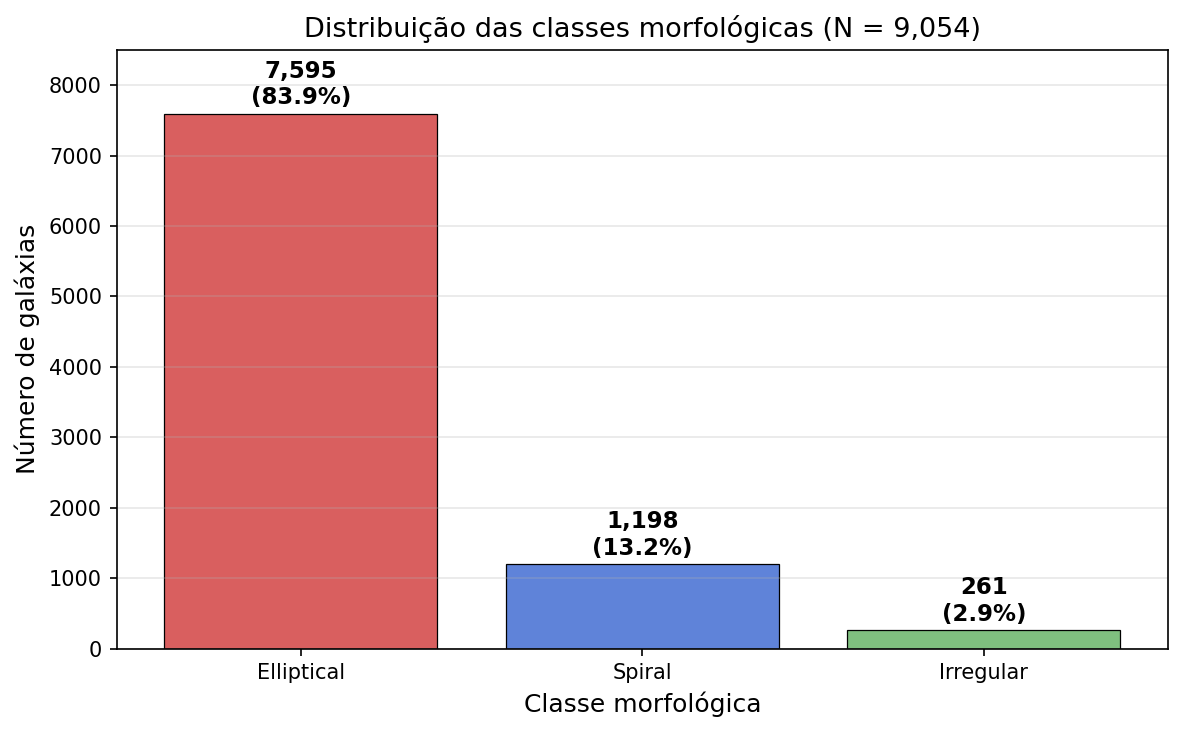
\includegraphics[width=0.85\textwidth]{fig01_distribuicao_classes.png}
  \caption{Distribuição das galáxias do catálogo por classe morfológica.}
  \label{fig:dist_classes}
\end{figure}

\begin{figure}[H]
  \centering
  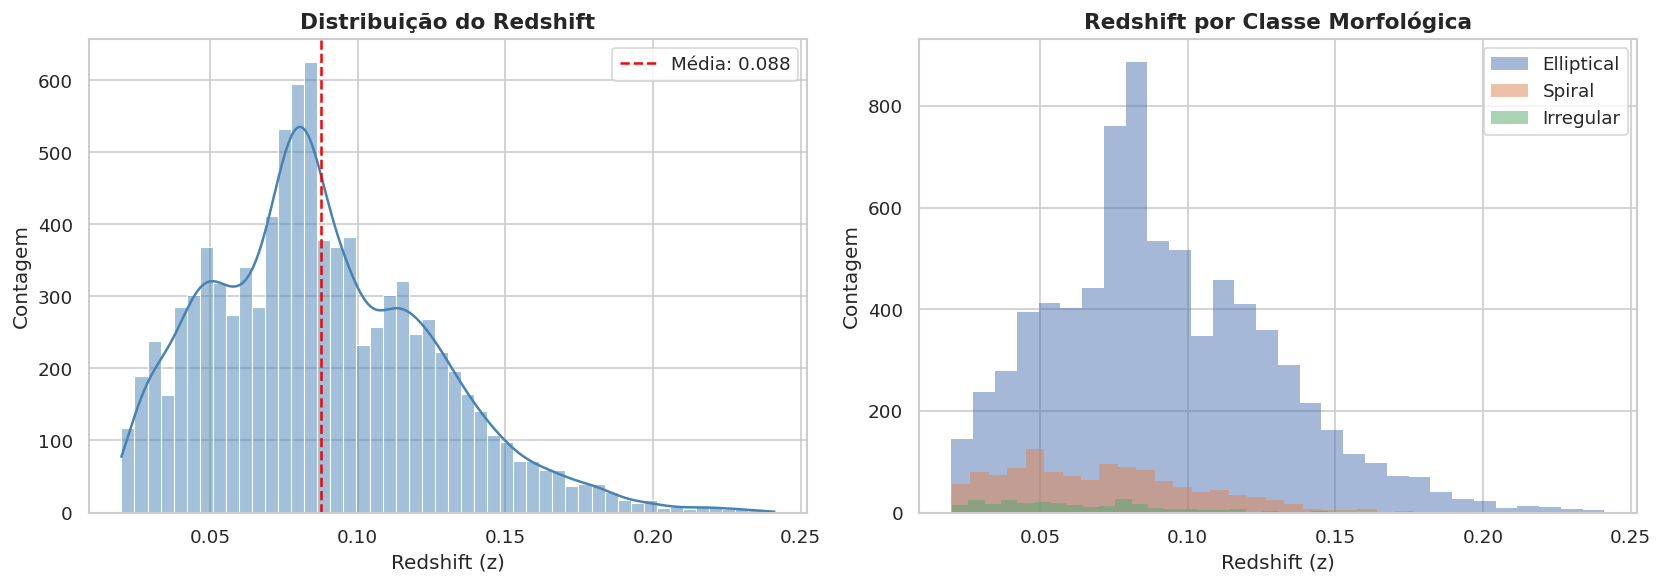
\includegraphics[width=0.85\textwidth]{fig02_distribuicao_redshift.png}
  \caption{Distribuição do \textit{redshift} espectroscópico por classe morfológica.}
  \label{fig:dist_redshift}
\end{figure}

A matriz de correlação entre as variáveis do catálogo, mostrada na
Figura~\ref{fig:corr_eda}, apresenta relações já esperadas. As
magnitudes em bandas adjacentes são quase colineares, com
$|\rho| > 0{,}98$, pois o brilho global domina sobre as diferenças de
cor. Os raios Petrosianos \texttt{petroR50} e \texttt{petroR90}
apresentam correlação negativa moderada com as magnitudes, com $\rho$
entre $-0{,}5$ e $-0{,}7$, o que confirma que galáxias mais luminosas
tendem a ser maiores. A dispersão de velocidades estelar
\texttt{velDisp} tem correlação positiva com os índices de cor, com
$\rho$ entre $0{,}67$ e $0{,}69$, em linha com a relação conhecida
entre massa estelar, profundidade do poço de potencial e idade das
populações estelares: galáxias mais massivas tendem a ser mais
vermelhas. A correlação entre \textit{redshift} e magnitudes brutas é fraca, o
que indica que o corte em magnitude limita o efeito de Malmquist
sobre as variáveis usadas.

\begin{figure}[H]
  \centering
  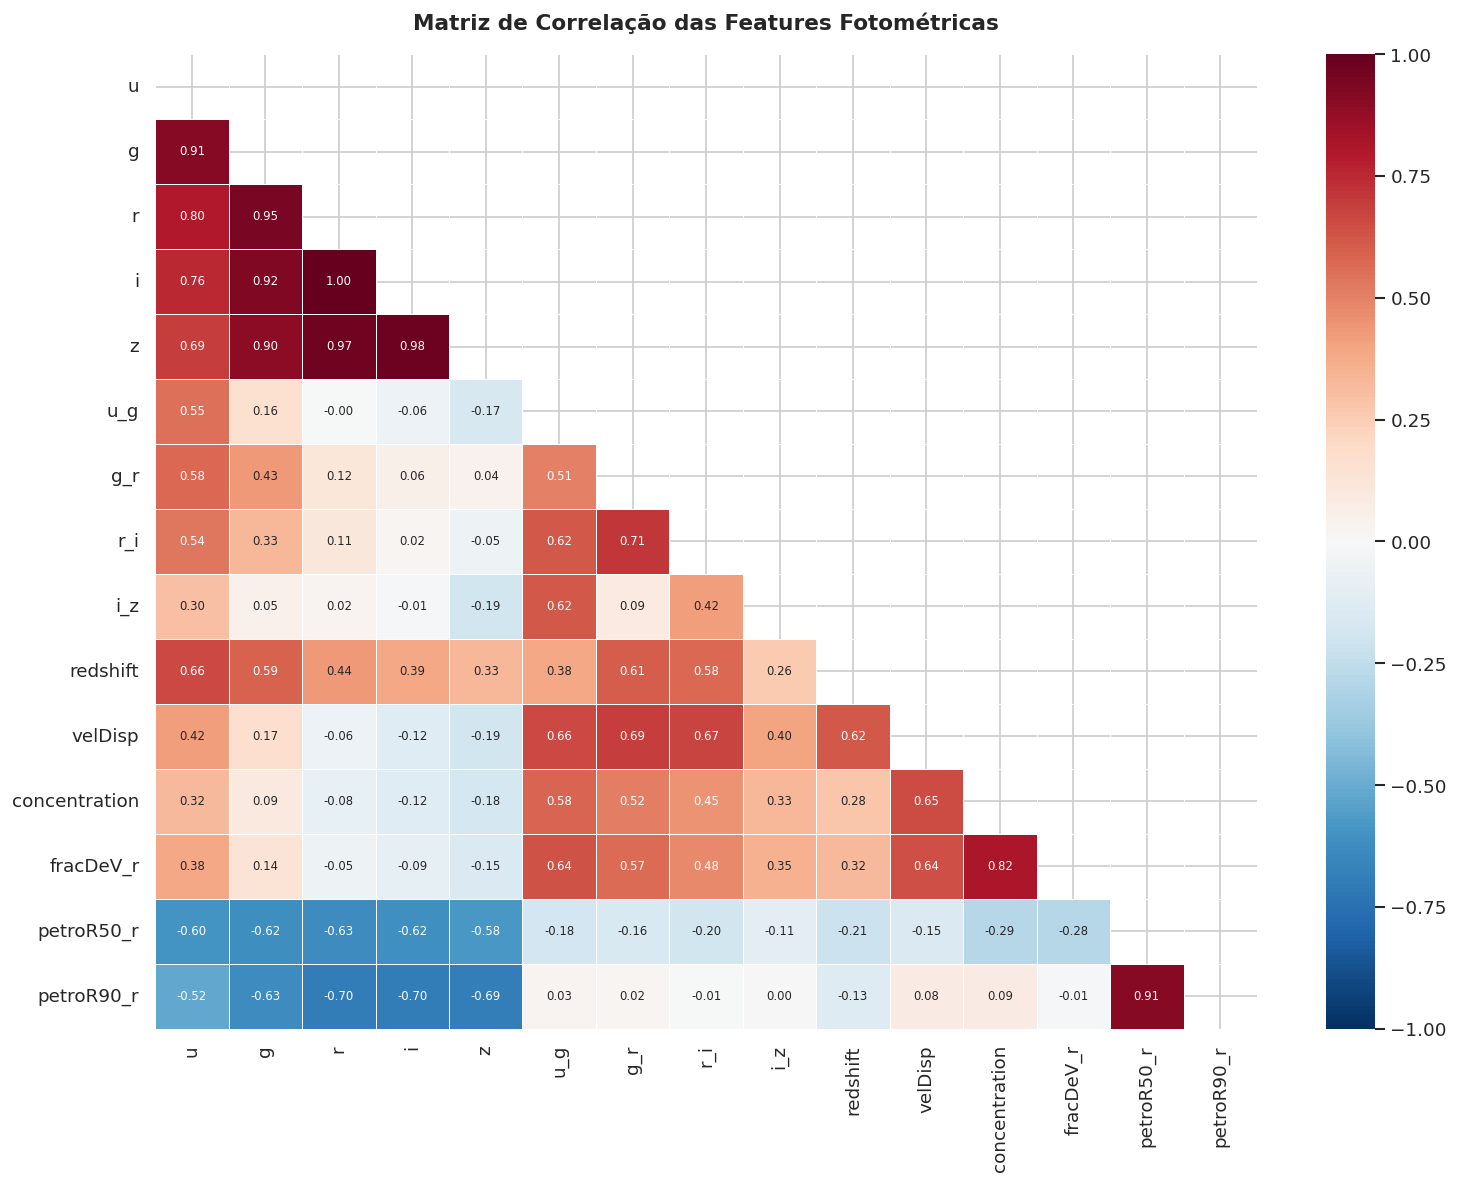
\includegraphics[width=0.85\textwidth]{fig05_matriz_correlacao.png}
  \caption{Matriz de correlação entre as variáveis do catálogo.}
  \label{fig:corr_eda}
\end{figure}

\subsection{Pré-processamento Aplicado}

Os índices de cor derivados, apresentados na
Figura~\ref{fig:indices_cor}, confirmam que $g-r$ é a combinação que
melhor separa espirais de elípticas, enquanto $i-z$ apresenta
distribuições quase iguais entre as três classes, com poder
discriminante muito baixo. O diagrama cor-concentração da
Figura~\ref{fig:cor_conc} mostra o mesmo comportamento em duas
dimensões. As elípticas tendem a ocupar a região superior-direita,
com cores mais vermelhas e perfis mais concentrados, mas a
sobreposição entre classes continua alta, em especial perto das
linhas $g-r = 0{,}7$ e $C = 3{,}0$. Nenhum corte binário em apenas
duas variáveis tabulares, portanto, gera uma separação limpa.

Entre as cinco \textit{features} estruturais derivadas, o índice de
concentração $C = R_{90}/R_{50}$ é a variável que mais separa as
classes individualmente. As medianas são $C \approx 2{,}97$ para
elípticas, $2{,}70$ para irregulares e $2{,}27$ para espirais,
seguindo a ordem esperada: quanto maior a dominância do bulge
central, maior o valor de $C$. Os intervalos interquartílicos ainda
se sobrepõem em parte, mas o deslocamento entre medianas é suficiente
para que a concentração esteja entre as variáveis mais úteis para a
classificação.

\begin{figure}[H]
  \centering
  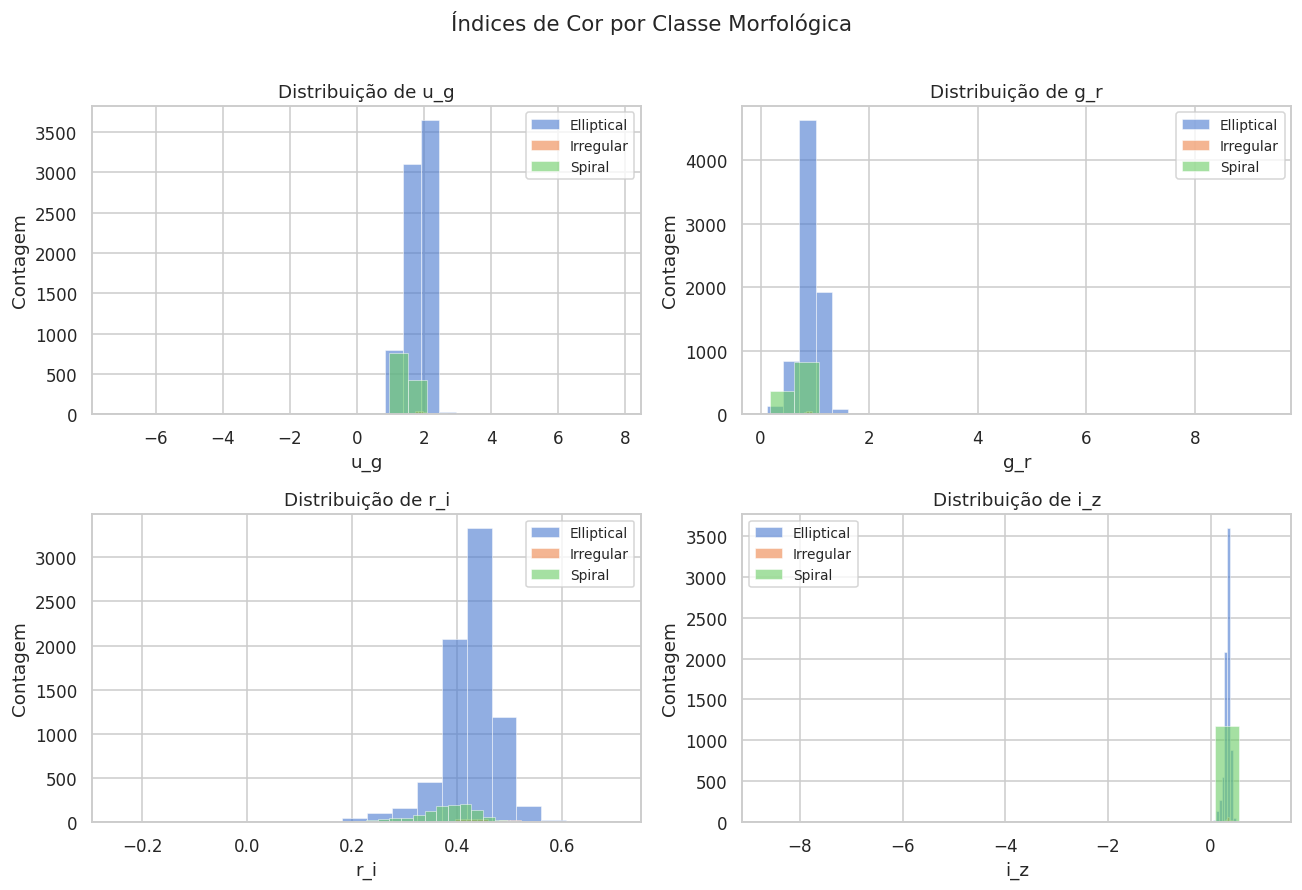
\includegraphics[width=\textwidth]{fig07_indices_cor_distribuicao.png}
  \caption{Distribuição dos índices de cor por classe morfológica. As
           galáxias elípticas apresentam cores consistentemente mais
           vermelhas.}
  \label{fig:indices_cor}
\end{figure}

\begin{figure}[H]
  \centering
  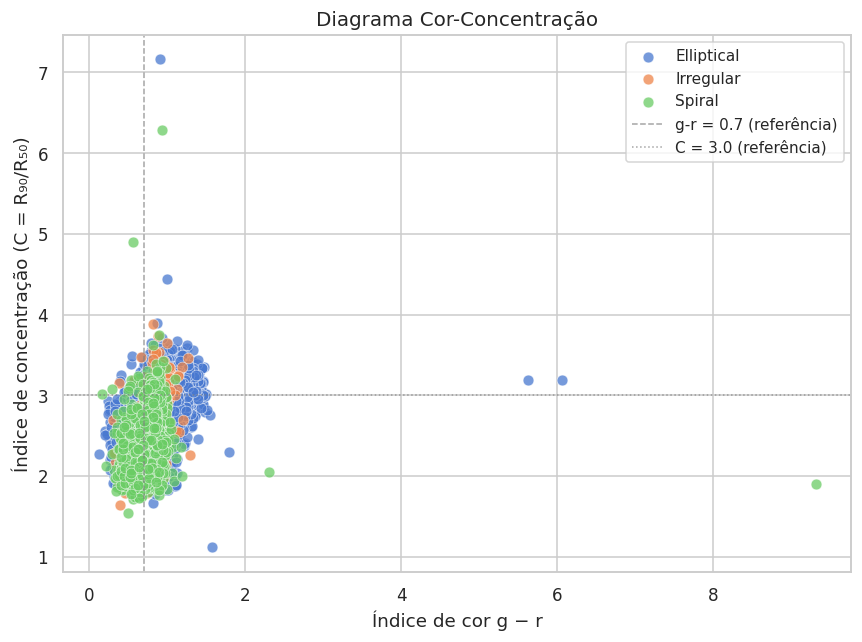
\includegraphics[width=0.75\textwidth]{fig09_cor_concentracao.png}
  \caption{Diagrama cor-concentração ($g-r$ \textit{vs.} $C = R_{90}/R_{50}$).
           As linhas tracejadas marcam os valores de referência $g-r = 0{,}7$
           e $C = 3{,}0$.}
  \label{fig:cor_conc}
\end{figure}

A matriz de correlação entre as 15 \textit{features} tabulares,
mostrada na Figura~\ref{fig:corr}, evidencia a alta colinearidade
entre as magnitudes brutas e os índices de cor construídos a partir
delas. Dois blocos adicionais aparecem na matriz. O par
\texttt{deVAB\_r}/\texttt{expAB\_r} apresenta redundância quase total,
com $\rho \approx 0{,}98$. A correlação entre \texttt{fracDeV\_r} e a
concentração é de $\rho \approx 0{,}82$, e ambas as variáveis estão
associadas à dominância do perfil de De Vaucouleurs no interior da
galáxia. A variável \texttt{velDisp} mantém correlação próxima de
$0{,}7$ com o índice $g-r$, o que reforça a relação cor-massa. O
\texttt{StandardScaler} aplicado antes do treinamento equaliza as
escalas das variáveis, mas não remove a colinearidade; as camadas
densas dos modelos absorvem essa redundância durante o aprendizado.

\begin{figure}[H]
  \centering
  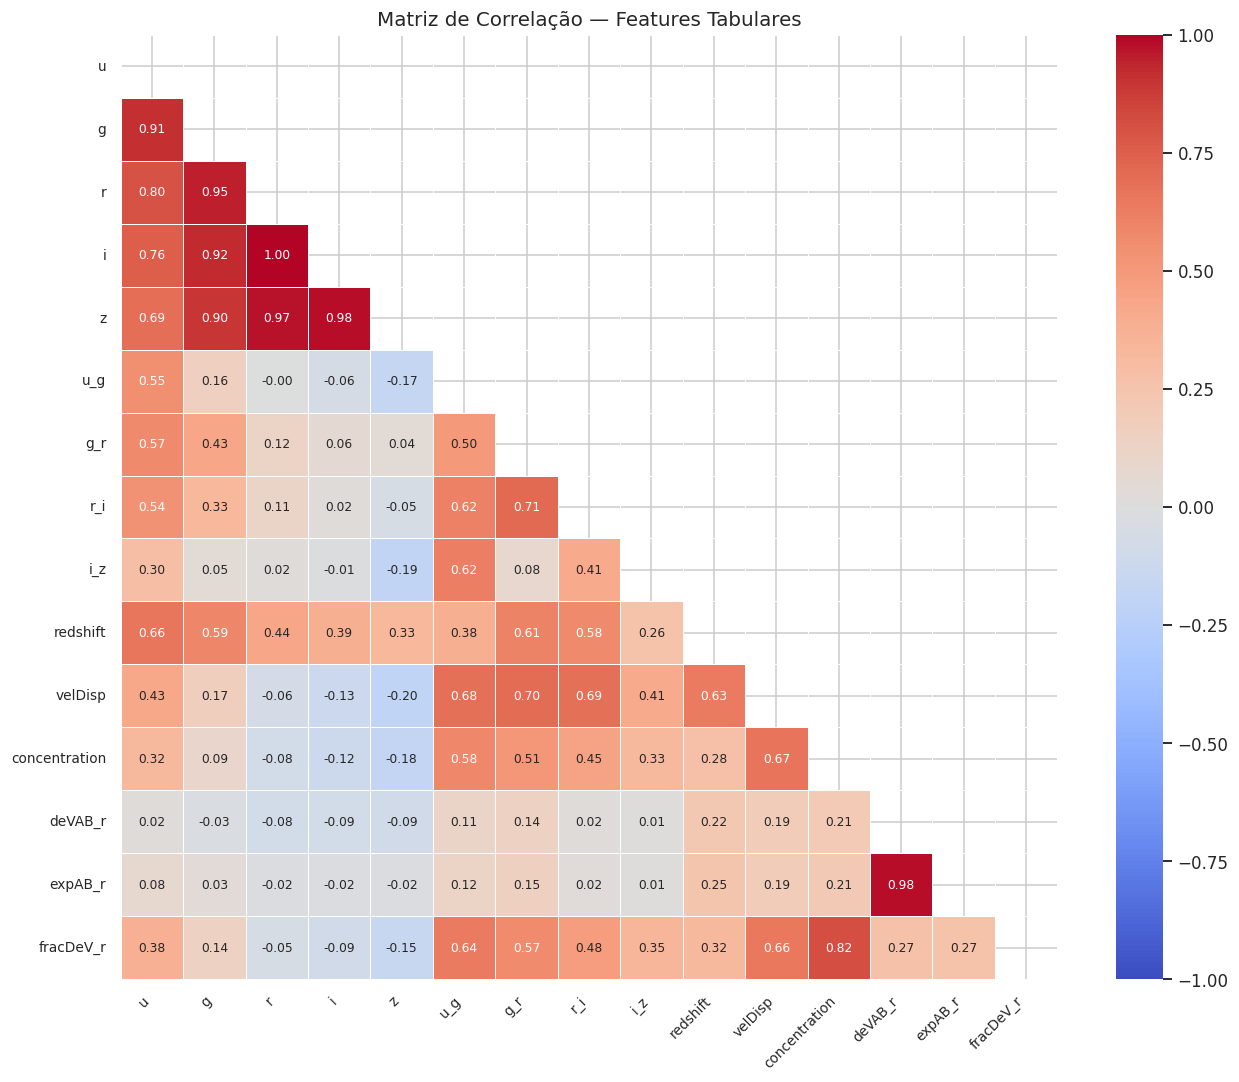
\includegraphics[width=\textwidth]{fig10_correlacao_features_tabulares.png}
  \caption{Matriz de correlação de Pearson entre as 15 \textit{features}
           tabulares.}
  \label{fig:corr}
\end{figure}

A Figura~\ref{fig:grid} traz um conjunto de imagens já
pré-processadas em composição RGB falsa-cor, na qual a banda $r$ é
mapeada no canal vermelho, $g$ no verde e $i$ no azul. Com o
\textit{arcsinh stretch} e a normalização por canal, as diferenças
morfológicas entre as classes ficam visíveis: as elípticas têm perfil
suave e simetria aproximada, as espirais mostram disco estendido com
subestruturas internas, e as irregulares apresentam morfologias
fragmentadas e assimétricas.

\begin{figure}[H]
  \centering
  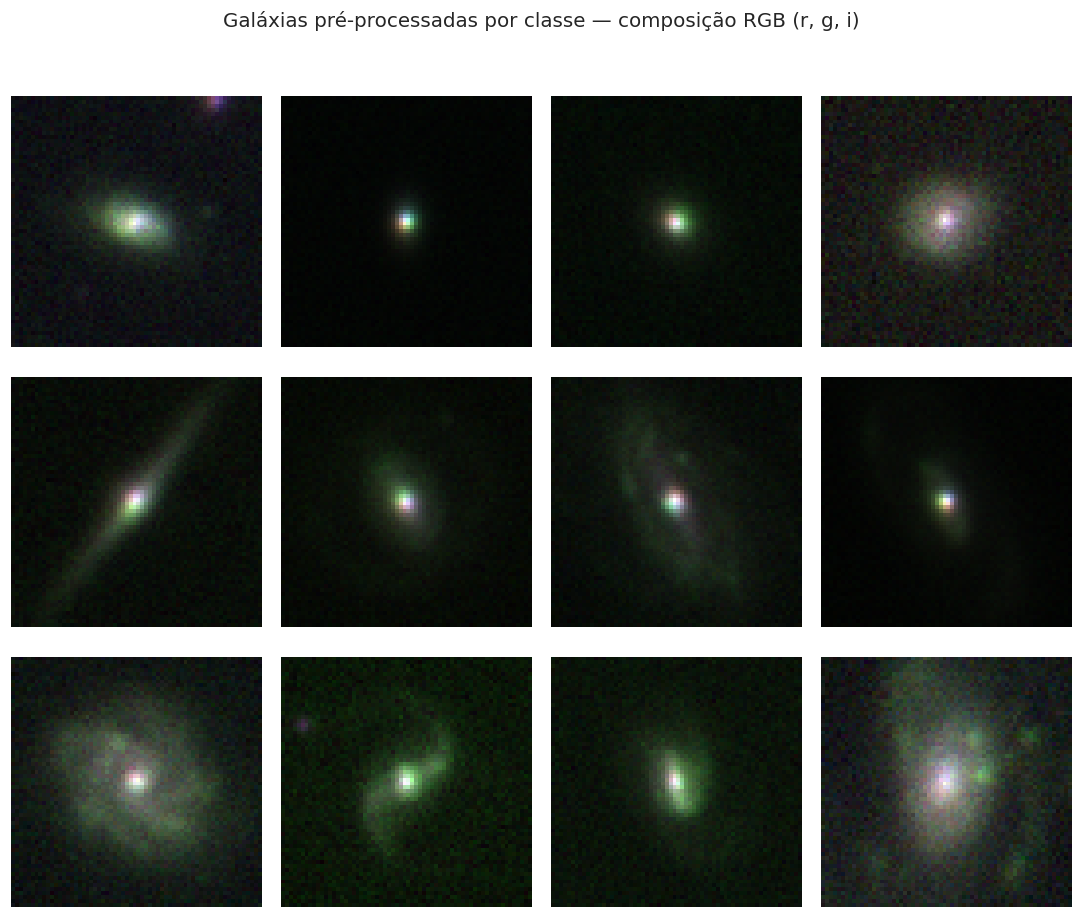
\includegraphics[width=\textwidth]{fig15_galaxy_grid_preprocessed.png}
  \caption{Grid de galáxias pré-processadas por classe morfológica, em
           composição RGB falsa-cor ($r$, $g$, $i$). Cada linha corresponde
           a uma classe e cada coluna a uma galáxia distinta.}
  \label{fig:grid}
\end{figure}

\subsection{Desempenho dos Modelos}

\subsubsection{MLP}

As curvas de treinamento do MLP, na Figura~\ref{fig:mlp_curves},
mostram convergência estável. A perda de validação cai rápido nas
primeiras épocas, fica próxima de 0,37 e o mecanismo de parada
antecipada, ou \textit{EarlyStopping}, restaura os melhores pesos por
volta da vigésima época. Nas primeiras iterações, a perda de validação
fica abaixo da perda de treino. Esse efeito é esperado porque o
\textit{dropout} atua apenas durante o treinamento e penaliza, por
isso, a métrica de treino.

\begin{figure}[H]
  \centering
  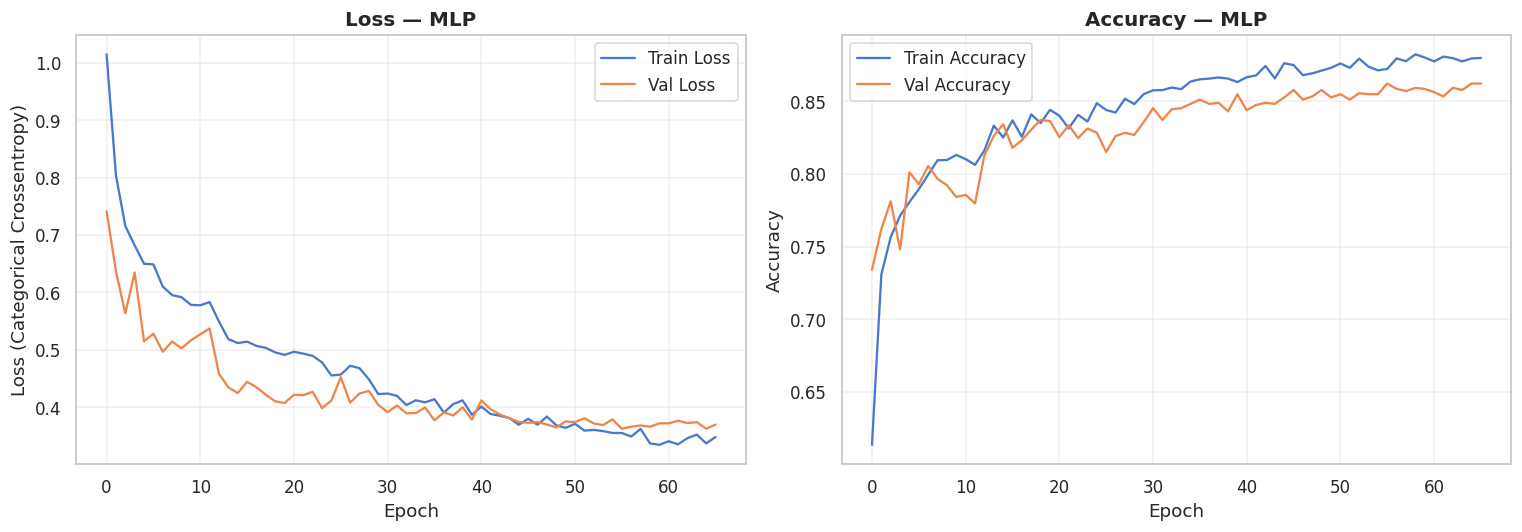
\includegraphics[width=\textwidth]{fig16_mlp_training_curves.png}
  \caption{Curvas de perda (esquerda) e acurácia (direita)
           do MLP ao longo das épocas de treinamento.}
  \label{fig:mlp_curves}
\end{figure}

\begin{figure}[H]
  \centering
  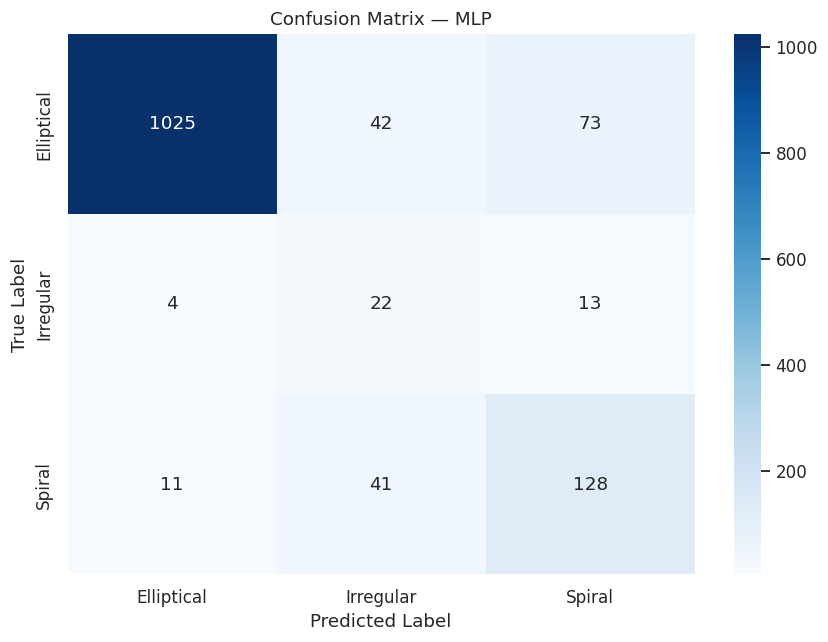
\includegraphics[width=0.7\textwidth]{fig17_mlp_confusion_matrix.png}
  \caption{Matriz de confusão do modelo MLP no conjunto de teste.}
  \label{fig:mlp_cm}
\end{figure}

O conjunto de teste reúne 1.359 galáxias, sendo 1.140 elípticas, 180
espirais e 39 irregulares. A matriz de confusão apresentada na
Figura~\ref{fig:mlp_cm} mostra um comportamento típico de um
classificador que usa apenas informação fotométrica. Das 39
irregulares, 22 são classificadas corretamente, a maior recuperação
entre os três modelos. Em troca, a pureza cai bastante: 41 espirais e
42 elípticas também recebem o rótulo \textit{Irregular}, e a
confiabilidade da classe fica em apenas 0,210. O principal foco de
erro está na confusão entre espirais e irregulares, duas classes que
ocupam faixas parcialmente sobrepostas no espaço de cor e
concentração. Sem informação visual, o MLP não consegue separá-las com
segurança. Na classe Elliptical, a confiabilidade é de 0,986 e a
completeza, de 0,899. Ou seja, quando o modelo prediz
\textit{Elliptical}, quase sempre acerta, mas deixa de identificar
cerca de um décimo das elípticas reais.

\subsubsection{CNN}

O treinamento da CNN, ilustrado na Figura~\ref{fig:cnn_curves}, é
mais instável que o do MLP. Durante as 40 épocas, a perda de treino
diminui gradualmente, enquanto a perda de validação oscila bastante e
chega a um pico próximo de 5,0 por volta da época 36, voltando depois
ao patamar anterior. Três fatores ajudam a explicar essa
instabilidade. O primeiro é o aumento artificial de dados, ou
\textit{data augmentation}, exemplificado na
Figura~\ref{fig:augmentation}, que introduz variabilidade a cada
\textit{batch}. O segundo é o baixo número de exemplos nas classes
raras, amplificado pelos pesos por classe, ou \textit{class weights}.
O terceiro é o tamanho reduzido do lote de validação, que torna a
métrica sensível a poucos exemplos difíceis. A acurácia de validação,
por outro lado, fica restrita a uma faixa estreita entre 0,85 e 0,90,
o que indica que as oscilações afetam sobretudo a confiança
probabilística das predições, e não a classe efetivamente atribuída.

\begin{figure}[H]
  \centering
  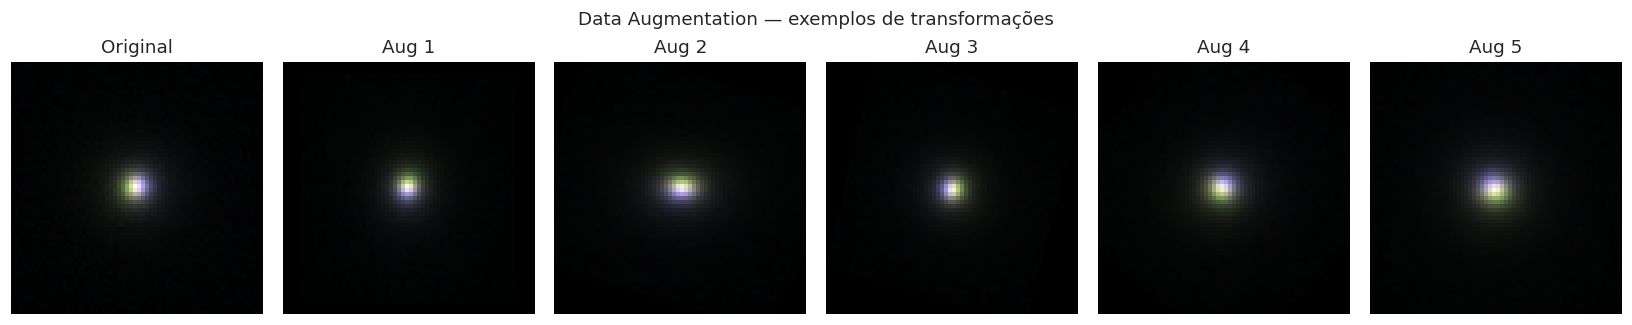
\includegraphics[width=\textwidth]{fig18_cnn_data_augmentation.png}
  \caption{Exemplos de \textit{data augmentation}: imagem original
           (esquerda) e versões transformadas por rotação, \textit{flips}
           e variações de brilho.}
  \label{fig:augmentation}
\end{figure}

\begin{figure}[H]
  \centering
  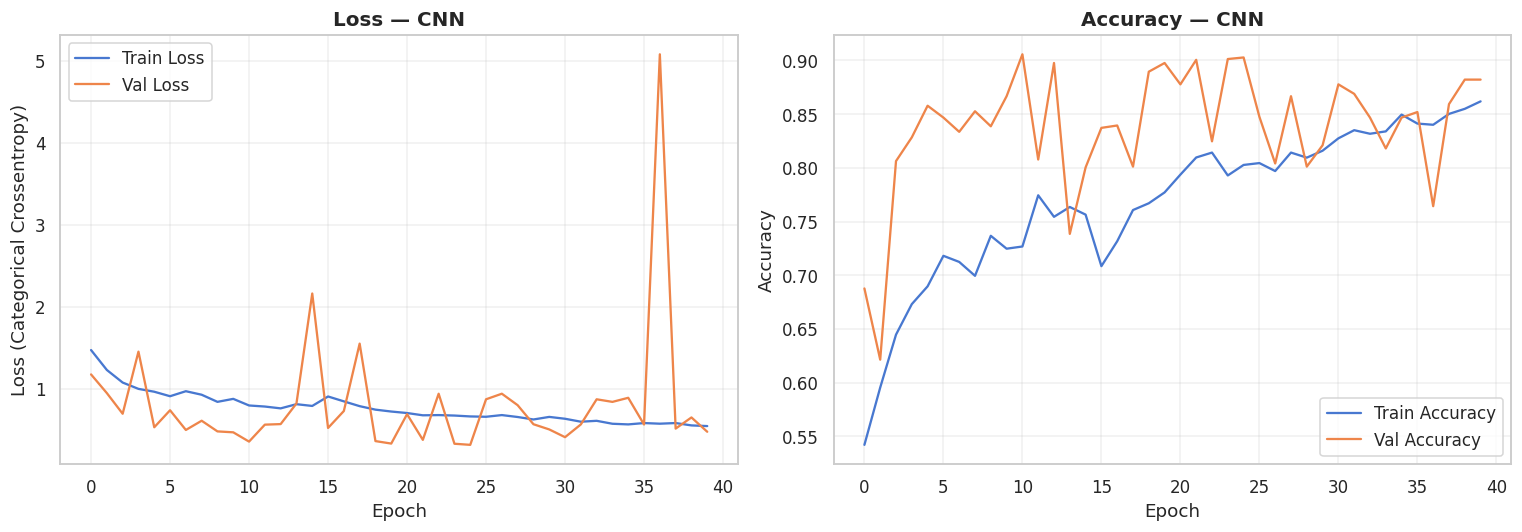
\includegraphics[width=\textwidth]{fig19_cnn_training_curves.png}
  \caption{Curvas de perda e acurácia do modelo CNN.}
  \label{fig:cnn_curves}
\end{figure}

\begin{figure}[H]
  \centering
  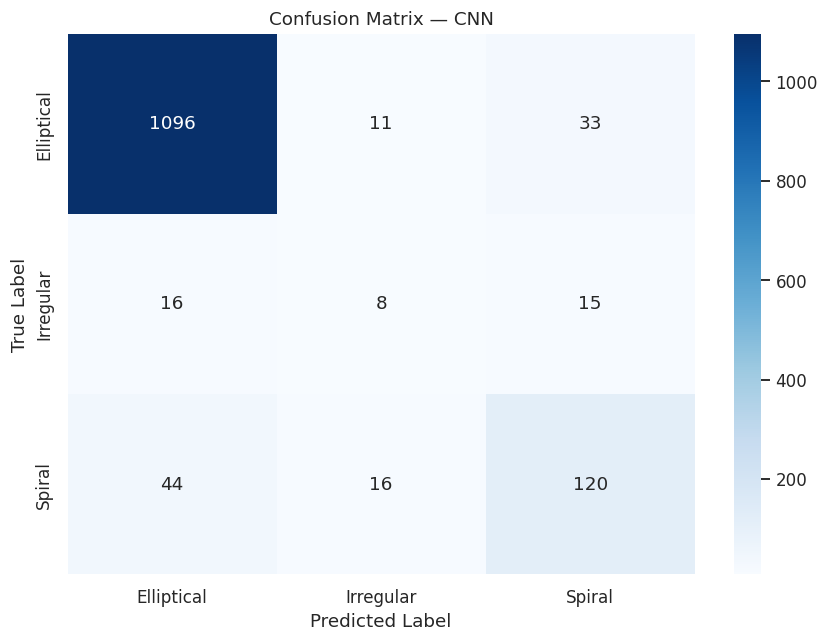
\includegraphics[width=0.7\textwidth]{fig17_cnn_confusion_matrix.png}
  \caption{Matriz de confusão do modelo CNN no conjunto de teste.}
  \label{fig:cnn_cm}
\end{figure}

A matriz de confusão correspondente, na Figura~\ref{fig:cnn_cm},
mostra o efeito desse regime instável. Em comparação com o MLP, a CNN
acerta 71 elípticas a mais, totalizando 1.096 contra 1.025, o que
explica o ganho de cerca de 3,6 pontos percentuais em acurácia. Esse
ganho, porém, se concentra na classe que já era a mais fácil de
identificar. Nas demais, o desempenho não melhora ou piora: a rede
recupera apenas 8 das 39 irregulares, contra 22 do MLP, e a
completeza em \textit{Spiral}, de 0,667, fica abaixo da obtida pelo
modelo tabular, de 0,711. Na prática, a CNN é mais conservadora e
atribui \textit{Elliptical} a boa parte das galáxias com morfologia
compacta e pouca estrutura visível, formato majoritário na amostra em
resolução $64\times 64$. O resultado é um F1-macro de 0,620, abaixo
do MLP e típico de classificadores que trocam equilíbrio entre classes
por acerto na classe dominante.

\subsubsection{Modelo Híbrido}

Ao juntar o ramo tabular ao convolucional, o treinamento do Híbrido,
mostrado na Figura~\ref{fig:hybrid_curves}, volta a ser estável. A
perda de validação converge em poucas épocas, o \textit{EarlyStopping}
encerra o ajuste em torno de 22 épocas e a diferença entre as curvas
de treino e de validação fica pequena ao longo de todo o processo. O
sinal tabular, formado por cor, concentração e dispersão de
velocidades, funciona como uma referência de baixa variância que
reduz o efeito do ruído das \textit{features} visuais extraídas em
baixa resolução.

\begin{figure}[H]
  \centering
  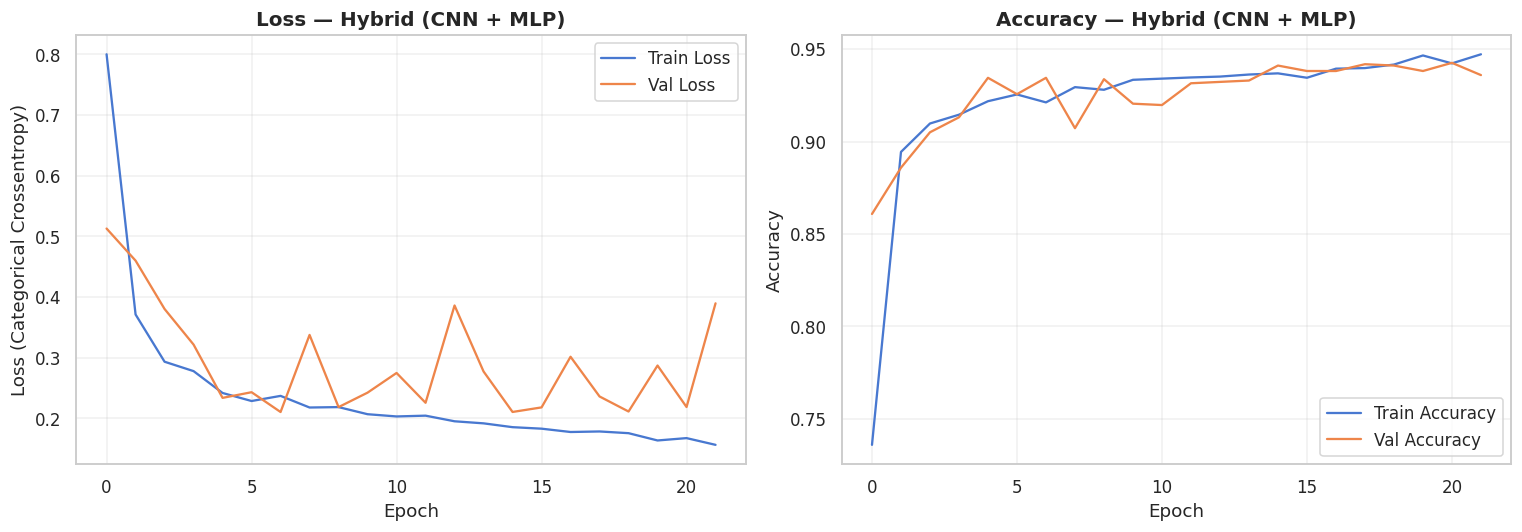
\includegraphics[width=\textwidth]{fig20_hybrid_training_curves.png}
  \caption{Curvas de treinamento do Híbrido (CNN + MLP).}
  \label{fig:hybrid_curves}
\end{figure}

\begin{figure}[H]
  \centering
  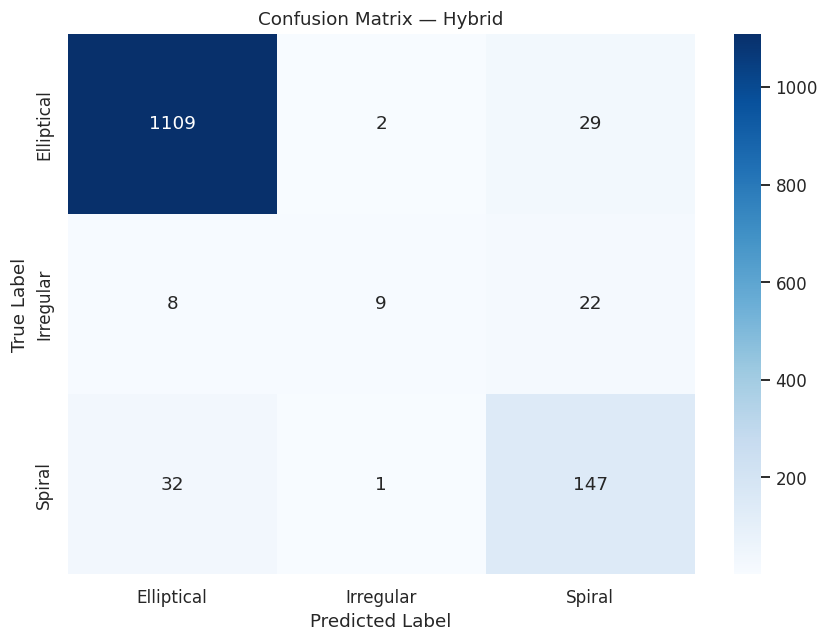
\includegraphics[width=0.7\textwidth]{fig17_hybrid_confusion_matrix.png}
  \caption{Matriz de confusão do Híbrido no conjunto de teste.}
  \label{fig:hybrid_cm}
\end{figure}

A matriz de confusão do Híbrido, apresentada na
Figura~\ref{fig:hybrid_cm}, traz o melhor resultado entre os três
modelos. O Híbrido classifica corretamente 1.109 elípticas, 147
espirais e 9 irregulares, totalizando 94 erros em 1.359 predições. Em
comparação com a CNN isolada, o maior ganho ocorre na classe
\textit{Spiral}, com 27 espirais a mais classificadas corretamente,
ou seja, 147 contra 120, sem aumento relevante de falsos positivos
entre as elípticas. Na classe Irregular, o Híbrido age de forma oposta
à do MLP: só atribui o rótulo \textit{Irregular} quando há indícios
fortes, o que gera apenas 12 predições nessa classe no conjunto de
teste, das quais 9 são acertos. A confiabilidade resultante, de
0,750, é bem maior que as do MLP, de 0,210, e da CNN, de 0,229, e
explica o valor de 0,700 em F1-macro, acima do MLP em mais de sete
pontos. Em um cenário desbalanceado, o F1-macro premia o equilíbrio
entre recuperação e pureza, que apenas o Híbrido consegue manter em
todas as classes.

\subsection{Análise Comparativa}

As métricas globais dos três modelos estão resumidas na
Tabela~\ref{tab:resultados_globais} e a análise por classe, com as métricas
astronômicas de completeza e confiabilidade, na
Tabela~\ref{tab:resultados_classe}. A Figura~\ref{fig:acc_f1} compara
graficamente as métricas globais, a Figura~\ref{fig:comp_rel} apresenta as
métricas por classe e a Figura~\ref{fig:cm_comparison} permite a comparação
visual das matrizes de confusão dos três modelos.

\begin{table}[H]
  \centering
  \caption{Métricas globais dos três modelos no conjunto de teste.}
  \label{tab:resultados_globais}
  \begin{tabular}{lccc}
    \toprule
    \textbf{Modelo} & \textbf{Acurácia} & \textbf{F1-macro} & \textbf{F1 ponderado} \\
    \midrule
    MLP (tabular)       & 0,865          & 0,632          & 0,884          \\
    CNN (imagens)       & 0,901          & 0,620          & 0,898          \\
    Híbrido (CNN + MLP) & \textbf{0,931} & \textbf{0,700} & \textbf{0,926} \\
    \bottomrule
  \end{tabular}
\end{table}

\begin{table}[H]
  \centering
  \caption{Completeza (Revocação) e Confiabilidade (Precisão) por classe morfológica.}
  \label{tab:resultados_classe}
  \begin{tabular}{ll ccc ccc}
    \toprule
    & & \multicolumn{3}{c}{\textbf{Completeza (Revocação)}} & \multicolumn{3}{c}{\textbf{Confiabilidade (Precisão)}} \\
    \cmidrule(lr){3-5} \cmidrule(lr){6-8}
    \textbf{Modelo} & & Ellip. & Irreg. & Spiral & Ellip. & Irreg. & Spiral \\
    \midrule
    MLP     & & 0,899 & 0,564 & 0,711 & 0,986 & 0,210 & 0,598 \\
    CNN     & & 0,961 & 0,205 & 0,667 & 0,948 & 0,229 & 0,714 \\
    Híbrido & & 0,973 & 0,231 & 0,817 & 0,965 & 0,750 & 0,742 \\
    \bottomrule
  \end{tabular}
\end{table}

\begin{figure}[H]
  \centering
  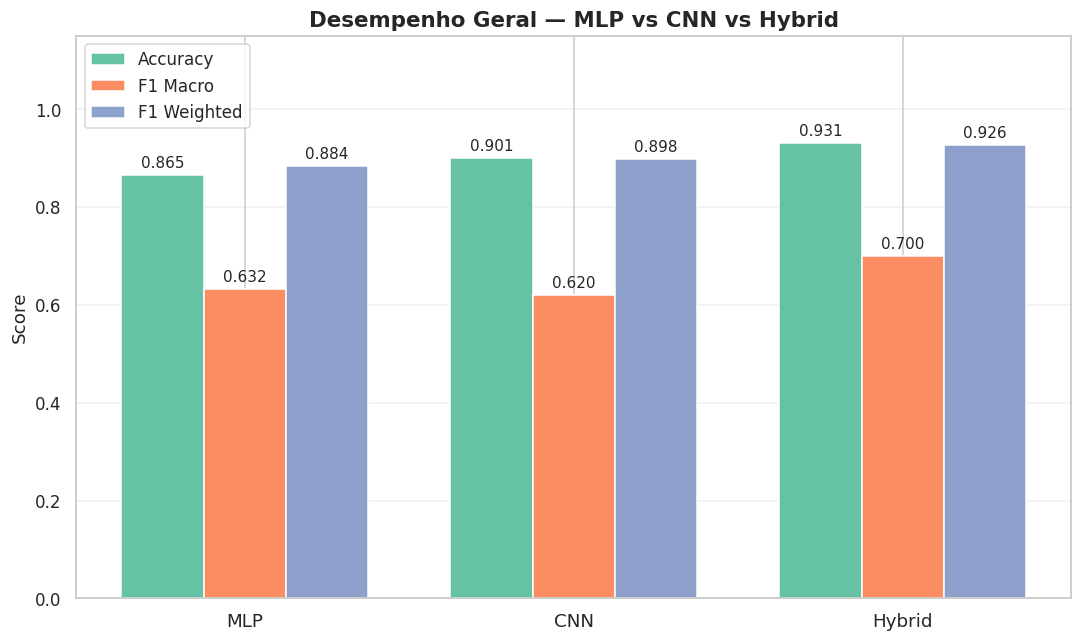
\includegraphics[width=\textwidth]{fig25_accuracy_f1_comparison.png}
  \caption{Comparação de acurácia, F1-macro e F1 ponderado entre
           os três modelos.}
  \label{fig:acc_f1}
\end{figure}

\begin{figure}[H]
  \centering
  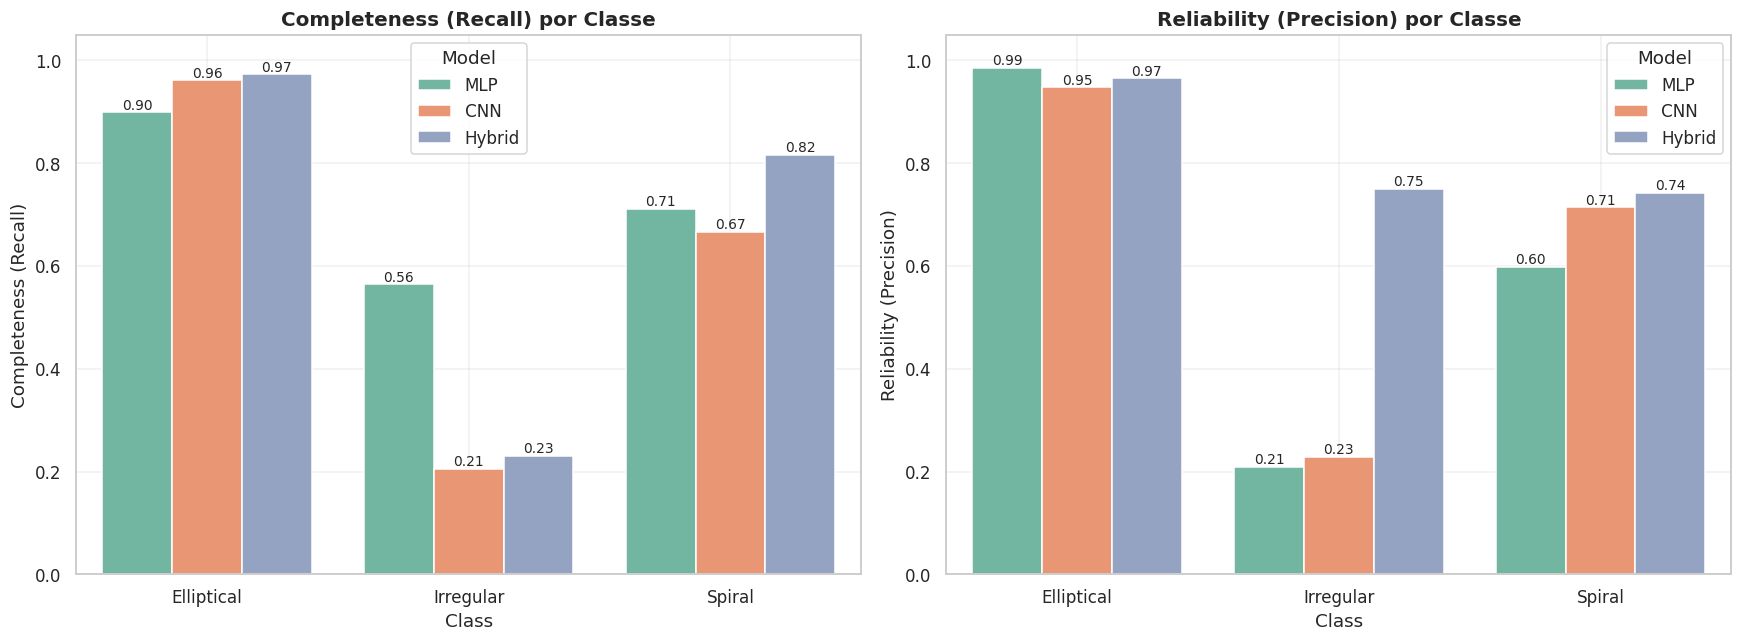
\includegraphics[width=\textwidth]{fig23_completeness_reliability_comparison.png}
  \caption{completeza e confiabilidade por classe
           morfológica e modelo.}
  \label{fig:comp_rel}
\end{figure}

\begin{figure}[H]
  \centering
  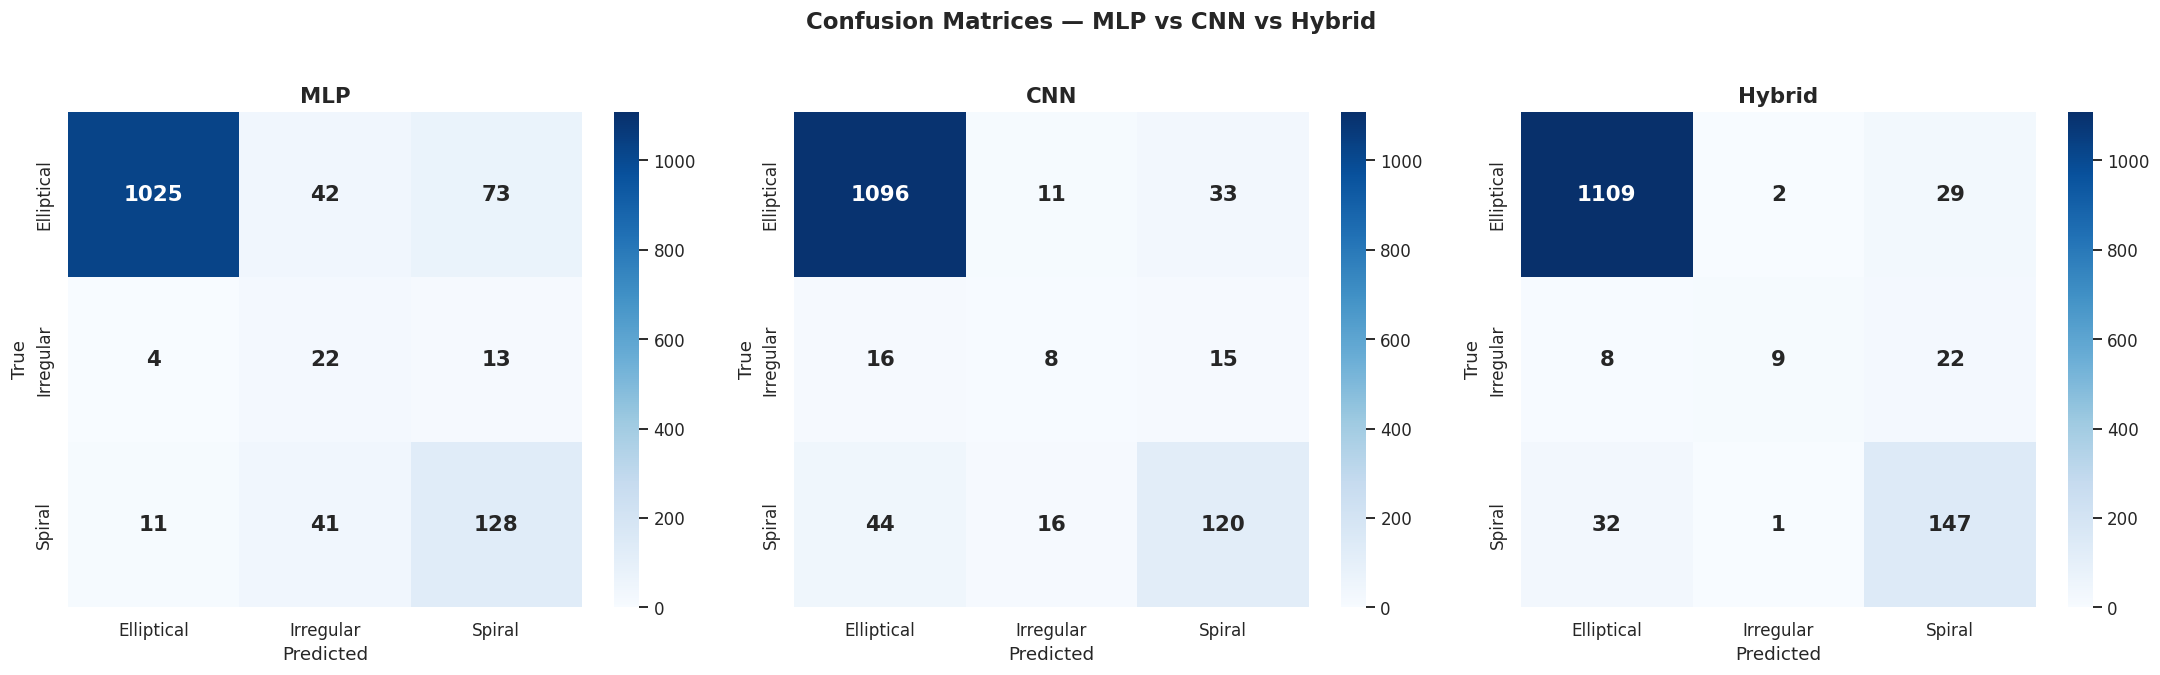
\includegraphics[width=\textwidth]{fig24_confusion_matrices_comparison.png}
  \caption{Matrizes de confusão dos três modelos na mesma escala de cor,
           permitindo comparação visual direta dos padrões de erro.}
  \label{fig:cm_comparison}
\end{figure}

A Tabela~\ref{tab:diagonal_cm} reúne a diagonal das três matrizes de
confusão e permite ler, diretamente, o número de acertos por classe em
relação ao total do conjunto de teste. Dessa comparação surgem três
padrões. Primeiro, o desempenho nas elípticas cresce do MLP ao Híbrido,
com ganho estável a cada incremento de informação. Em segundo lugar,
as espirais não se beneficiam da CNN isolada e só apresentam melhora
clara quando as duas modalidades são combinadas. Por fim, a classe
Irregular continua sendo o ponto fraco das três arquiteturas: mesmo no
melhor caso, pouco mais da metade dos exemplos é recuperada. O
principal gargalo da classificação morfológica automática, portanto,
está na classe rara, e não na classe dominante.

\begin{table}[H]
  \centering
  \caption{Galáxias corretamente classificadas por classe (diagonal das
           matrizes de confusão) em relação ao total por classe no
           conjunto de teste.}
  \label{tab:diagonal_cm}
  \begin{tabular}{lccc}
    \toprule
    \textbf{Classe (total)} & \textbf{MLP} & \textbf{CNN} & \textbf{Híbrido} \\
    \midrule
    Elliptical (1.140) & 1.025 (89,9\%) & 1.096 (96,1\%) & \textbf{1.109 (97,3\%)} \\
    Spiral (180)       & 128 (71,1\%)   & 120 (66,7\%)   & \textbf{147 (81,7\%)}   \\
    Irregular (39)     & \textbf{22 (56,4\%)} & 8 (20,5\%) & 9 (23,1\%)       \\
    \midrule
    Total (1.359)      & 1.175 (86,5\%) & 1.224 (90,1\%) & \textbf{1.265 (93,1\%)} \\
    \bottomrule
  \end{tabular}
\end{table}

A Tabela~\ref{tab:complexidade} relaciona o número aproximado de
parâmetros de cada modelo com as métricas globais. A CNN tem cerca de
50 vezes mais parâmetros que o MLP, e o Híbrido soma, ao ramo
convolucional, o ramo tabular e a camada de fusão. Do MLP para a CNN,
a acurácia sobe de 0,865 para 0,901, um acréscimo de 3,6 pontos
percentuais, mas o F1-macro recua de 0,632 para 0,620. Esse padrão
mostra que o ganho de acerto global da CNN vem da classificação mais
agressiva da classe majoritária, e não de uma melhora distribuída
entre as demais. O Híbrido, com cerca de 700 mil parâmetros a mais do
que a CNN, aumenta tanto a acurácia, que passa para 0,931, quanto o
F1-macro, que chega a 0,700. Esse resultado sugere que a combinação
de informação visual e tabular produz um classificador mais
equilibrado do que cada modalidade isolada.

\begin{table}[H]
  \centering
  \caption{Relação entre complexidade dos modelos e desempenho.}
  \label{tab:complexidade}
  \begin{tabular}{lcccc}
    \toprule
    \textbf{Modelo} & \textbf{Parâmetros} & \textbf{Acurácia} & \textbf{F1-macro} & \textbf{F1 ponderado} \\
    \midrule
    MLP     & $\sim$47 mil  & 0,865          & 0,632          & 0,884          \\
    CNN     & $\sim$2,5 M   & 0,901          & 0,620          & 0,898          \\
    Híbrido & $\sim$3,2 M   & \textbf{0,931} & \textbf{0,700} & \textbf{0,926} \\
    \bottomrule
  \end{tabular}
\end{table}

Olhar apenas para a acurácia seria enganoso neste caso. Um
classificador trivial que classificasse todas as galáxias como
\textit{Elliptical} já chegaria a 0,839, o que reduz o intervalo útil
de comparação entre modelos. É por isso que a CNN, mesmo superior ao
MLP em acurácia, fica abaixo dele em F1-macro, com 0,620 contra
0,632: a métrica, baseada na média harmônica por classe, penaliza o
comportamento que a acurácia premia, ou seja, ignorar as classes
raras.

Ao cruzar as Tabelas~\ref{tab:resultados_globais},
\ref{tab:resultados_classe} e~\ref{tab:diagonal_cm}, o papel de cada
modalidade fica mais claro. A fotometria pré-calculada pelo
\textit{pipeline} do SDSS carrega boa parte da informação morfológica
útil. Por isso, o MLP, com cerca de 47 mil parâmetros, consegue uma
\textit{baseline} sólida e até supera, em F1-macro, uma CNN cinquenta
vezes maior. A rota visual isolada ajuda sobretudo a refinar a
fronteira entre elípticas e espirais, mas, sem o apoio das variáveis
tabulares, tende a colapsar a classe Irregular sobre a majoritária.
Só quando as duas modalidades são combinadas, como no Híbrido, o
classificador se mantém preciso na classe dominante, competitivo na
intermediária e parcimonioso, porém confiável, na classe rara. A
escolha entre modelos depende, portanto, do \textit{trade-off}
desejado entre cobertura e pureza das classes minoritárias: o MLP
prioriza a cobertura, o Híbrido prioriza a pureza, e a CNN isolada
não é a melhor opção em nenhuma das duas dimensões.

\subsection{Interpretabilidade}

A Figura~\ref{fig:gradcam} mostra que o ramo convolucional do Híbrido
produz padrões de ativação diferentes para cada classe morfológica.
Nas elípticas, os mapas se concentram na região central, em linha com
o perfil de brilho suave e dominado pelo bulge. Nas espirais, a
ativação se estende ao longo do disco, com maior intensidade em
regiões assimétricas, onde braços e núcleos de formação estelar
produzem contraste local. Nas irregulares, os mapas ficam mais
dispersos, o que é compatível com a morfologia fragmentada dessas
galáxias.

Essa correspondência qualitativa é encorajadora, mas exige duas
ressalvas. A primeira diz respeito à resolução das imagens, de
$64\times 64$ pixels, nas quais as galáxias ocupam poucas dezenas de
pixels, o que limita a identificação de estruturas morfológicas finas
mesmo para um observador humano. Os mapas de ativação atuam, portanto,
sobre imagens com pouca informação estrutural. A segunda é de natureza
metodológica: o Grad-CAM aponta as regiões que mais contribuem para a
classe prevista, mas não é uma explicação causal formal e não garante
correspondência direta entre as \textit{features} aprendidas pela
rede e propriedades físicas reais das galáxias.

\begin{figure}[H]
  \centering
  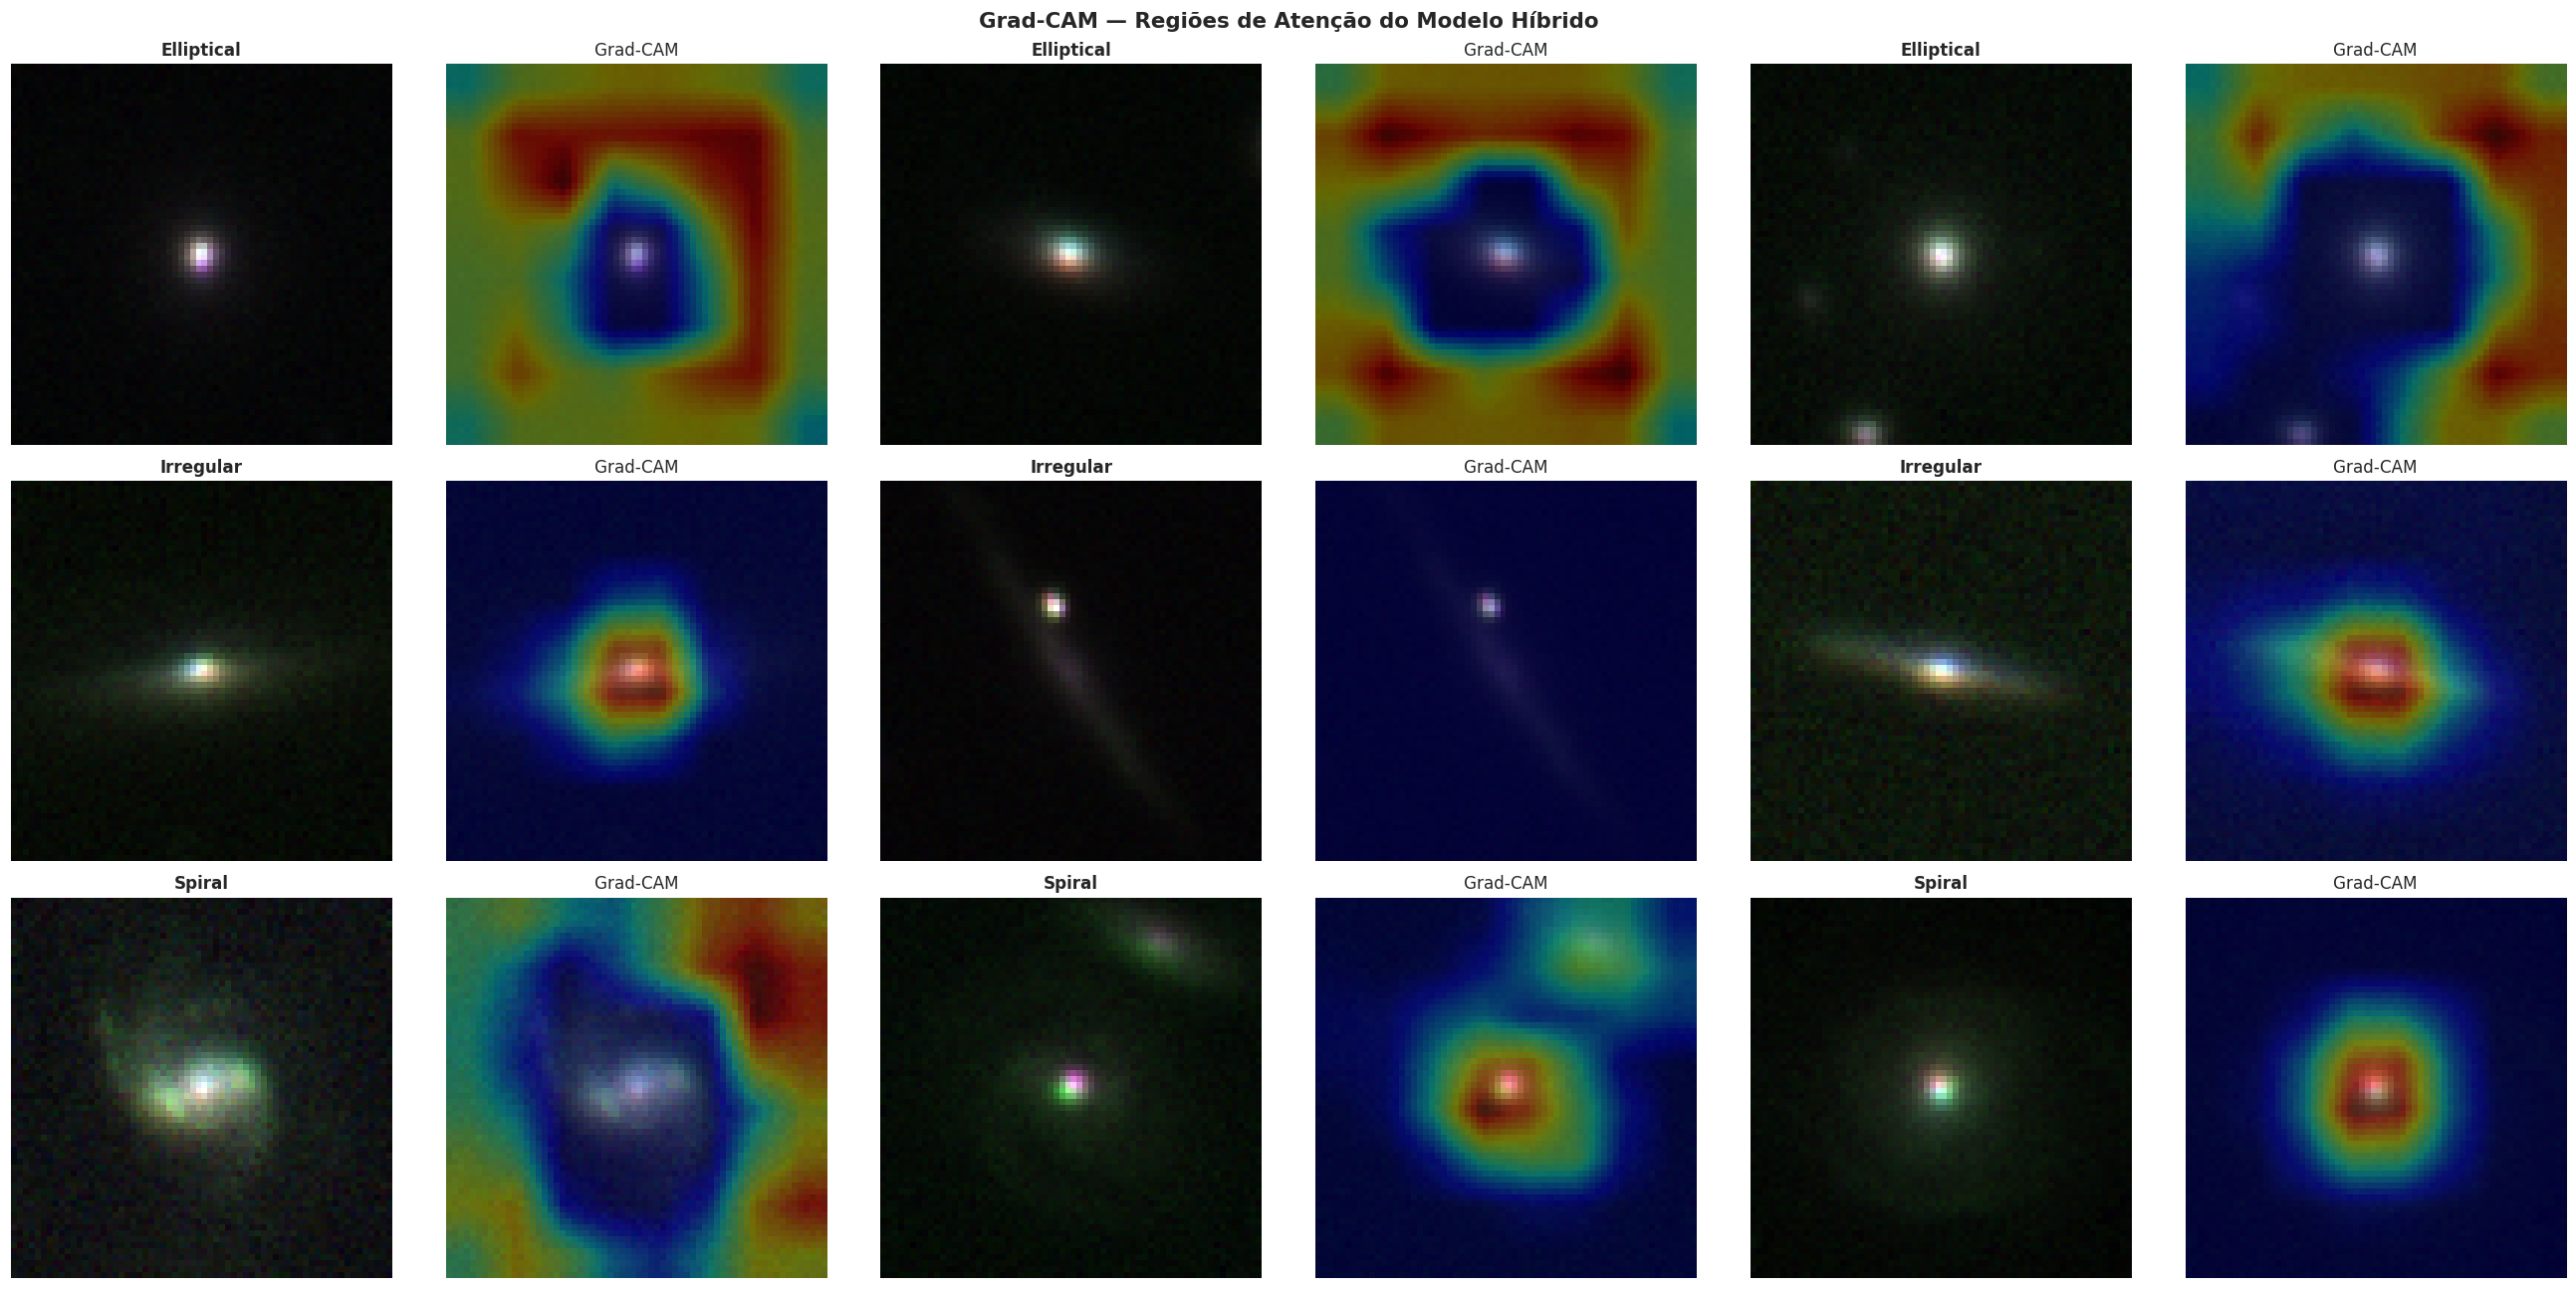
\includegraphics[width=\textwidth]{fig21_hybrid_gradcam.png}
  \caption{Grad-CAM do Híbrido para exemplos de cada classe
           morfológica. Cada par mostra a imagem RGB original (esquerda) e
           a sobreposição do mapa de calor Grad-CAM (direita). Regiões
           quentes indicam maior contribuição para a classificação.}
  \label{fig:gradcam}
\end{figure}

\subsection{Galáxias Mal Classificadas}

A Figura~\ref{fig:misclassified} mostra exemplos de galáxias
classificadas de forma errada pelo Híbrido, junto com o desvio
padronizado de cada \textit{feature} tabular em relação à média da
classe predita. Três padrões de erro aparecem nos casos apresentados.
No primeiro, uma galáxia espiral tem morfologia visual compacta e
perfil suave, que a aproximam das elípticas, e suas \textit{features}
tabulares se afastam pouco dos valores típicos dessa classe. No
segundo, uma irregular tem perfil fotométrico alongado, porém
aproximadamente simétrico, com valores de concentração e cor
compatíveis com elíptica, o que leva o modelo ao mesmo erro. No
terceiro, uma irregular predita como espiral tem uma fonte compacta
acompanhada de uma companheira próxima, padrão que sugere sistema em
interação.

Em todos os casos, as \textit{features} tabulares do objeto mal
classificado ficam a menos de $2\sigma$ das médias da classe predita.
Isso indica que os erros refletem ambiguidade real entre morfologia e
fotometria, e não ruído simples de rotulagem. O padrão é compatível
com a incerteza dos próprios rótulos do Galaxy Zoo 2, cujo critério
de consenso, com $f \geq 0{,}8$, já foi pensado para afastar os casos
mais ambíguos do conjunto de treinamento.

\begin{figure}[H]
  \centering
  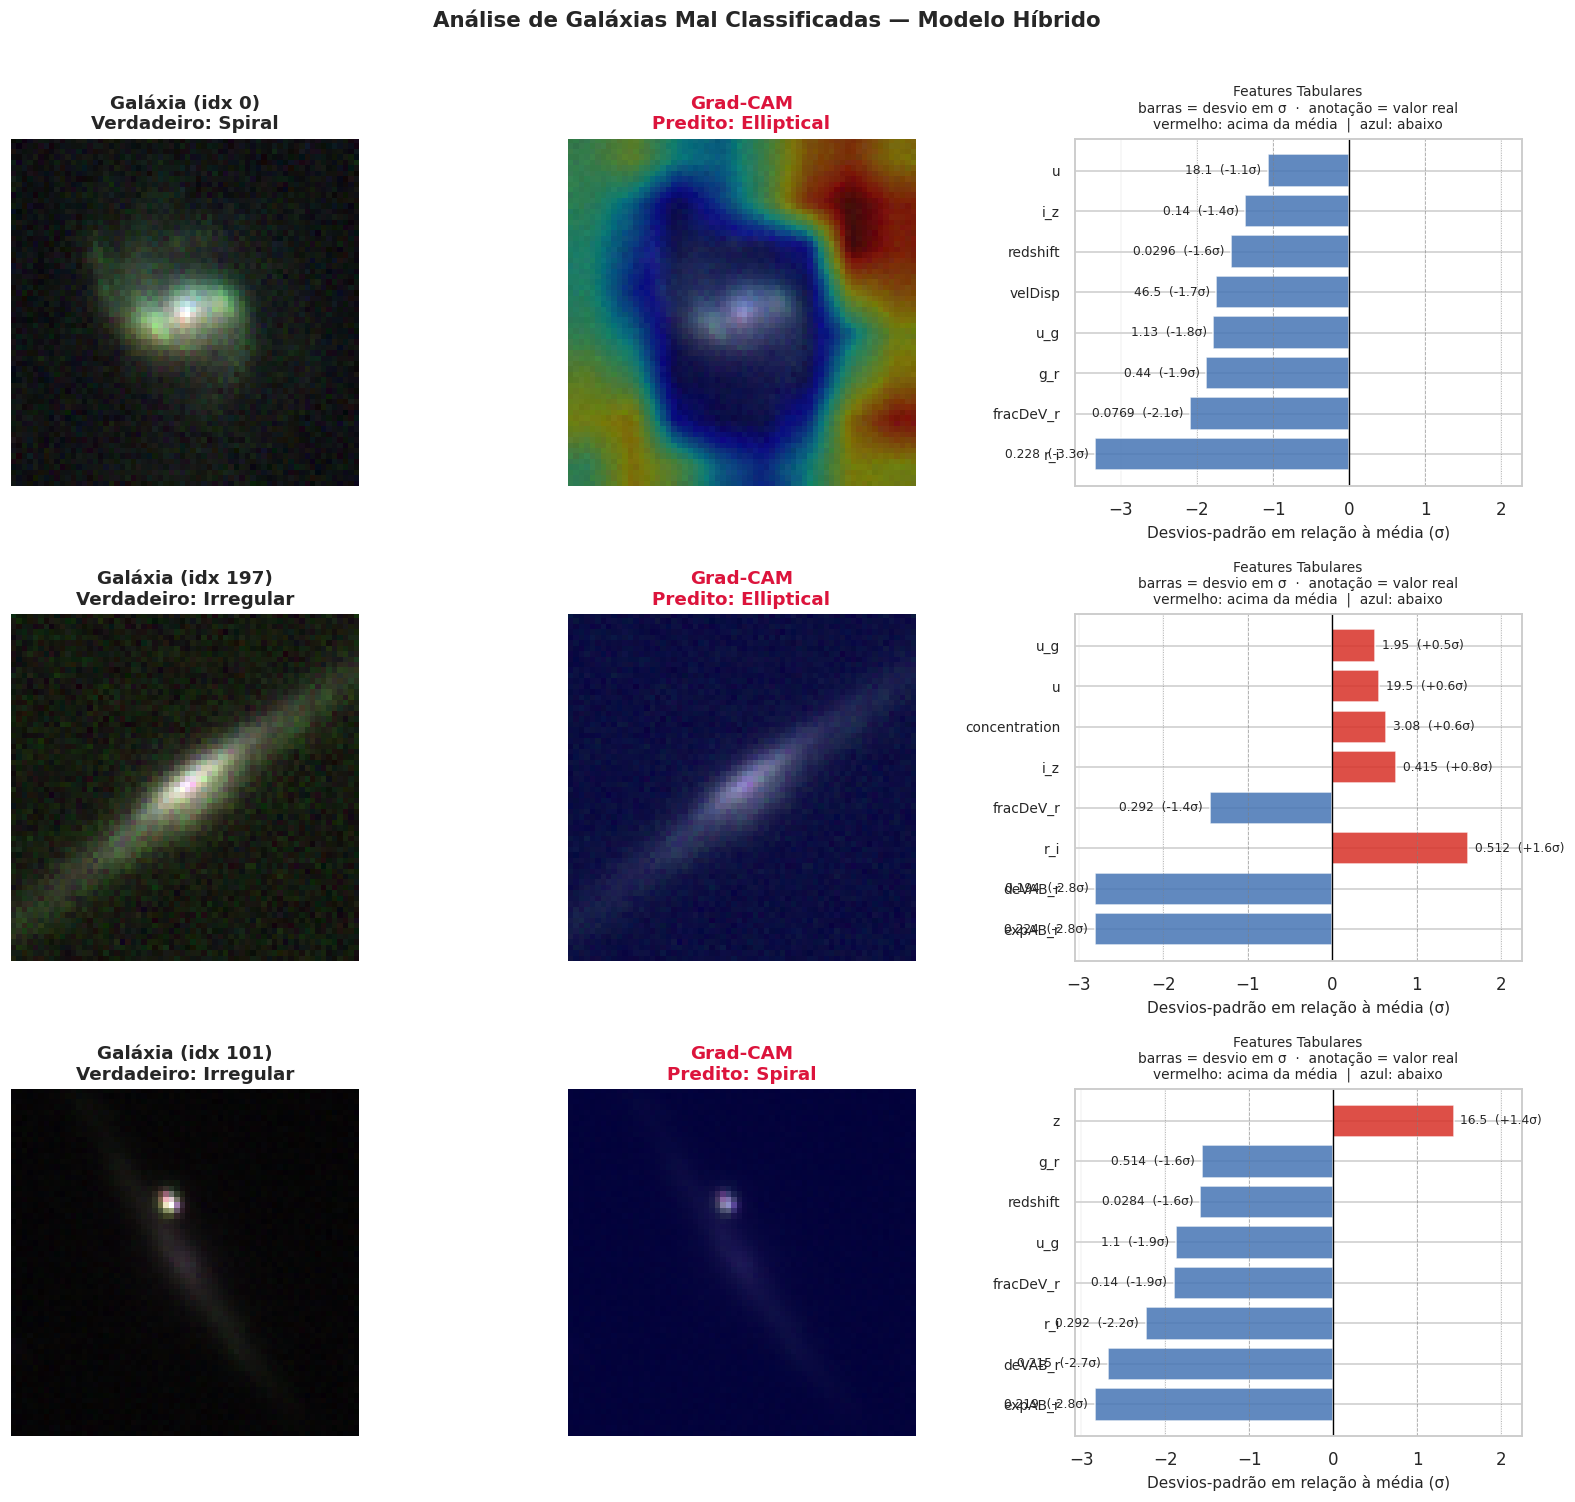
\includegraphics[width=\textwidth]{fig26_misclassified_galaxies.png}
  \caption{Exemplos de galáxias mal classificadas pelo Híbrido.
           Cada imagem indica a classe verdadeira (\textit{True}) e a
           classe predita (\textit{Pred}). Os casos representativos
           mostram morfologias ambíguas onde visual e fotometria apontam
           para classes distintas.}
  \label{fig:misclassified}
\end{figure}

\subsection{Limitações}

Os resultados apresentados têm algumas limitações. A primeira é o
desbalanceamento entre classes. Mesmo com o uso de \textit{class
weights}, a classe Irregular, com 261 exemplos no catálogo completo,
continua sendo o principal gargalo dos três modelos. A segunda
limitação é a estratégia de avaliação: todos os resultados vêm de uma
única partição 70/15/15, gerada com semente fixa. Uma análise mais
rigorosa em termos estatísticos pediria validação cruzada
estratificada, capaz de fornecer intervalos de confiança para as
métricas. A terceira limitação está nos rótulos. Os dados do Galaxy
Zoo 2, apesar da boa qualidade, carregam incerteza própria da
classificação visual, e o critério adotado, com $f \geq 0{,}8$ e
$N_\text{votos} \geq 20$, exclui uma parcela considerável de galáxias
cuja classe seria ambígua. Reduzir esses limiares aumentaria a
amostra, com o custo previsível de rótulos mais ruidosos.

% ─────────────────────────────────────────────────────────────────────────────
\section{Conclusão}
% ─────────────────────────────────────────────────────────────────────────────

O projeto GalaxyNet construiu um \textit{pipeline} reprodutível de
classificação morfológica de galáxias a partir de dados do SDSS DR17 e do
Galaxy Zoo 2, implementou três arquiteturas de \textit{deep learning}
(MLP, CNN e Híbrido) e realizou a avaliação comparativa dos modelos
sobre um conjunto de teste comum. O catálogo final contém 9.054 galáxias,
descritas por 15 \textit{features} tabulares e por imagens $64 \times 64$
nas bandas $g$, $r$ e $i$.

A comparação entre os modelos mostra um padrão que não é trivial.
Usando apenas as \textit{features} tabulares, o MLP forneceu uma
\textit{baseline} com acurácia de 0,865 e F1-macro de 0,632, além da
maior sensibilidade para a classe Irregular, com completeza de 0,564,
ainda que com baixa precisão de 0,210. A CNN chegou a acurácia
superior, de 0,901, mas F1-macro de 0,620, abaixo do MLP, o que
mostra que a rede convolucional favorece a classe dominante e não
generaliza bem para as irregulares. O Híbrido foi o único modelo que
aumentou, ao mesmo tempo, a acurácia para 0,931, o F1-macro para
0,700 e o F1 ponderado para 0,926, além de obter a melhor completeza
e confiabilidade nas espirais e a maior pureza nas irregulares, com
confiabilidade de 0,750.

Esses resultados sugerem que, com os dados usados, a informação visual
complementa as \textit{features} fotométricas pré-calculadas e que a
fusão tardia produz um classificador mais estável do que cada
modalidade isolada. O fato de a CNN, sozinha, não superar o MLP em
F1-macro indica que as variáveis tabulares carregam informação
morfológica que as imagens brutas em baixa resolução não conseguem
recuperar por conta própria. A análise Grad-CAM mostrou que as regiões
de atenção do Híbrido são compatíveis com a morfologia esperada para
cada classe, o que reforça, dentro dos limites da técnica, a
interpretação de que as representações aprendidas refletem padrões
astrofísicos plausíveis.

As limitações estão concentradas no desbalanceamento entre classes,
no número reduzido de exemplos na classe Irregular (261 objetos) e no
uso de uma única partição de treino, validação e teste. Como direções
futuras, podem-se explorar técnicas de \textit{transfer learning} a
partir de modelos pré-treinados em catálogos maiores, como o
Galaxy10 DECaLS, o uso de validação cruzada estratificada para
estimar intervalos de confiança nas métricas e um ajuste dos limiares
de consenso do Galaxy Zoo 2, com o objetivo de ampliar a amostra das
classes minoritárias.

% ─────────────────────────────────────────────────────────────────────────────
\begin{thebibliography}{9}

\bibitem{hart2016}
Hart, R.~E. et al. (2016).
\textit{Galaxy Zoo 2: detailed morphological classifications for 304,122 galaxies from the Sloan Digital Sky Survey}.
Monthly Notices of the Royal Astronomical Society, 445(4), 3466--3486.
\url{https://doi.org/10.1093/mnras/stu1816}

\bibitem{conselice2003}
Conselice, C.~J. (2003).
\textit{The Relationship between Stellar Light Distributions of Galaxies and Their Formation Histories}.
The Astrophysical Journal Supplement Series, 147(1), 1--28.
\url{https://doi.org/10.1086/375001}

\bibitem{chawla2002}
Chawla, N.~V., Bowyer, K.~W., Hall, L.~O., \& Kegelmeyer, W.~P. (2002).
\textit{SMOTE: Synthetic Minority Over-sampling Technique}.
Journal of Artificial Intelligence Research, 16, 321--357.
\url{https://doi.org/10.1613/jair.953}

\bibitem{lupton2004}
Lupton, R., Blanton, M.~R., Fekete, G., et al. (2004).
\textit{Preparing Red-Green-Blue Images from CCD Data}.
Publications of the Astronomical Society of the Pacific, 116(816), 133--137.
\url{https://doi.org/10.1086/382245}

\bibitem{selvaraju2017}
Selvaraju, R.~R., Cogswell, M., Das, A., et al. (2017).
\textit{Grad-CAM: Visual Explanations from Deep Networks via Gradient-based Localization}.
International Conference on Computer Vision (ICCV), 618--626.
\url{https://doi.org/10.1109/ICCV.2017.74}

\bibitem{sdss_dr17}
Abdurrouf et al. (2022).
\textit{The Seventeenth Data Release of the Sloan Digital Sky Surveys: Complete Release of MaNGA, MaStar, and APOGEE-2 Data}.
The Astrophysical Journal Supplement Series, 259(2), 35.
\url{https://doi.org/10.3847/1538-4365/ac4414}

\bibitem{dieleman2015}
Dieleman, S., Willett, K.~W., \& Dambre, J. (2015).
\textit{Rotation-invariant convolutional neural networks for galaxy morphology prediction}.
Monthly Notices of the Royal Astronomical Society, 450(2), 1441--1459.
\url{https://doi.org/10.1093/mnras/stv632}

\bibitem{kingma2014}
Kingma, D.~P. \& Ba, J. (2015).
\textit{Adam: A Method for Stochastic Optimization}.
International Conference on Learning Representations (ICLR).
\url{https://arxiv.org/abs/1412.6980}

\bibitem{goodfellow2016}
Goodfellow, I., Bengio, Y., \& Courville, A. (2016).
\textit{Deep Learning}.
MIT Press. Capítulo 8: Optimization for Training Deep Models.
\url{https://www.deeplearningbook.org}

\bibitem{simonyan2014}
Simonyan, K. \& Zisserman, A. (2015).
\textit{Very Deep Convolutional Networks for Large-Scale Image Recognition}.
International Conference on Learning Representations (ICLR).
\url{https://arxiv.org/abs/1409.1556}

\bibitem{srivastava2014}
Srivastava, N., Hinton, G., Krizhevsky, A., Sutskever, I., \& Salakhutdinov, R. (2014).
\textit{Dropout: A Simple Way to Prevent Neural Networks from Overfitting}.
Journal of Machine Learning Research, 15(56), 1929--1958.
\url{https://jmlr.org/papers/v15/srivastava14a.html}

\bibitem{hubble1926}
Hubble, E.~P. (1926).
\textit{Extragalactic Nebulae}.
Astrophysical Journal, 64, 321--369.
\url{https://ui.adsabs.harvard.edu/abs/1926ApJ....64..321H}

\bibitem{devaucouleurs1959}
de Vaucouleurs, G. (1959).
\textit{Classification and Morphology of External Galaxies}.
In: Handbuch der Physik, ed.\ S.~Flügge (Berlin: Springer), 53, 275.

\bibitem{conselice2014}
Conselice, C.~J. (2014).
\textit{The Evolution of Galaxy Structure Over Cosmic Time}.
Annual Review of Astronomy and Astrophysics, 52, 291--337.
\url{https://doi.org/10.1146/annurev-astro-081913-040037}

\bibitem{kravtsov2012}
Kravtsov, A.~V. \& Borgani, S. (2012).
\textit{Formation of Galaxy Clusters}.
Annual Review of Astronomy and Astrophysics, 50, 353--409.
\url{https://doi.org/10.1146/annurev-astro-081811-125502}

\bibitem{allen2011}
Allen, S.~W., Evrard, A.~E., \& Mantz, A.~B. (2011).
\textit{Cosmological Parameters from Observations of Galaxy Clusters}.
Annual Review of Astronomy and Astrophysics, 49, 409--470.
\url{https://doi.org/10.1146/annurev-astro-081710-102514}

\bibitem{dressler1980}
Dressler, A. (1980).
\textit{Galaxy Morphology in Rich Clusters: Implications for the Formation and Evolution of Galaxies}.
Astrophysical Journal, 236, 351--365.
\url{https://doi.org/10.1086/157753}

\bibitem{postman1984}
Postman, M. \& Geller, M.~J. (1984).
\textit{The Morphology-Density Relation: The Group Connection}.
Astrophysical Journal, 281, 95.
\url{https://ui.adsabs.harvard.edu/abs/1984ApJ...281...95P}

\bibitem{dressler1997}
Dressler, A., Oemler, A.~J., Couch, W., et al. (1997).
\textit{Evolution since z = 0.5 of the Morphology-Density Relation for Clusters of Galaxies}.
Astrophysical Journal, 490, 577.
\url{https://doi.org/10.1086/304890}

\bibitem{boselli2022}
Boselli, A., Fossati, M., \& Sun, M. (2022).
\textit{Ram Pressure Stripping in High-Density Environments}.
The Astronomy and Astrophysics Review, 30, 3.
\url{https://doi.org/10.1007/s00159-022-00140-3}

\bibitem{peng2010}
Peng, Y., Maiolino, R., Cochrane, R., et al. (2010).
\textit{Mass and Environment as Drivers of Galaxy Evolution in SDSS and zCOSMOS and the Origin of the Schechter Function}.
Astrophysical Journal, 721, 193--221.
\url{https://doi.org/10.1088/0004-637X/721/1/193}

\bibitem{nair2010}
Nair, P.~B. \& Abraham, R.~G. (2010).
\textit{A Catalog of Detailed Visual Morphological Classifications for 14,034 Galaxies in the Sloan Digital Sky Survey}.
Astrophysical Journal Supplement Series, 186, 427.
\url{https://doi.org/10.1088/0067-0049/186/2/427}

\bibitem{lintott2008}
Lintott, C.~J., Schawinski, K., Slosar, A., et al. (2008).
\textit{Galaxy Zoo: Morphologies Derived from Visual Inspection of Galaxies from the Sloan Digital Sky Survey}.
Monthly Notices of the Royal Astronomical Society, 389, 1179.
\url{https://doi.org/10.1111/j.1365-2966.2008.13689.x}

\bibitem{willett2013}
Willett, K.~W., Lintott, C.~J., Bamford, S.~P., et al. (2013).
\textit{Galaxy Zoo 2: Detailed Morphological Classifications for 304,122 Galaxies from the Sloan Digital Sky Survey}.
Monthly Notices of the Royal Astronomical Society, 435, 2835--2860.
\url{https://doi.org/10.1093/mnras/stt1458}

\bibitem{dominguez2018}
Domínguez Sánchez, H., Huertas-Company, M., Bernardi, M., Tuccillo, D., \& Fischer, J.~L. (2018).
\textit{Improving Galaxy Morphologies for SDSS with Deep Learning}.
Monthly Notices of the Royal Astronomical Society, 476, 3661--3676.
\url{https://doi.org/10.1093/mnras/sty338}

\bibitem{walmsley2022}
Walmsley, M., Lintott, C., Geréb, K., et al. (2022).
\textit{Galaxy Zoo DECaLS: Detailed Visual Morphology Measurements from Volunteers and Deep Learning for 314,000 Galaxies}.
Monthly Notices of the Royal Astronomical Society, 509, 3966--3988.
\url{https://doi.org/10.1093/mnras/stab2093}

\bibitem{huertascompany2023}
Huertas-Company, M. \& Lanusse, F. (2023).
\textit{The DAWES Review 10: The Impact of Deep Learning for the Analysis of Galaxy Surveys}.
Publications of the Astronomical Society of Australia, 40, e001.
\url{https://doi.org/10.1017/pasa.2022.55}

\bibitem{york2000}
York, D.~G. et al. (2000).
\textit{The Sloan Digital Sky Survey: Technical Summary}.
Astronomical Journal, 120, 1579--1587.
\url{https://doi.org/10.1086/301513}

\bibitem{tukey1977}
Tukey, J.~W. (1977).
\textit{Exploratory Data Analysis}.
Addison-Wesley Publishing Company, Reading, MA.

\end{thebibliography}

\end{document}
